%# -*- coding:utf-8 -*-
%%%%%%%%%%%%%%%%%%%%%%% file template.tex %%%%%%%%%%%%%%%%%%%%%%%%%
%
% This is a general template file for the LaTeX package SVJour3
% for Springer journals.          Springer Heidelberg 2010/09/16
%
% Copy it to a new file with a new name and use it as the basis
% for your article. Delete % signs as needed.
%
% This template includes a few options for different layouts and
% content for various journals. Please consult a previous issue of
% your journal as needed.
%
%%%%%%%%%%%%%%%%%%%%%%%%%%%%%%%%%%%%%%%%%%%%%%%%%%%%%%%%%%%%%%%%%%%
%
%
\RequirePackage{fix-cm}
%
%\documentclass{svjour3}                     % onecolumn (standard format)
%\documentclass[smallcondensed]{svjour3}     % onecolumn (ditto)
%\documentclass[smallextended]{svjour3}       % onecolumn (second format)
\documentclass[twocolumn]{svjour3}          % twocolumn
%
\smartqed  % flush right qed marks, e.g. at end of proof
%
\usepackage{graphicx}
\usepackage{mathptmx}      % use Times fonts if available on your
\usepackage{latexsym}
\usepackage[ruled]{algorithm2e}
%\usepackage{algorithm}
\usepackage{algorithmic}
\usepackage{amssymb}
\usepackage{amsmath}
\usepackage{mathrsfs}
\usepackage{txfonts}
\usepackage{subfigure}
\usepackage{float}
\usepackage{balance}
\usepackage[misc]{ifsym}
\usepackage{textcomp}
\usepackage[svgnames,rgb]{xcolor}
\usepackage{pdfcomment}
\usepackage{makecell}
\usepackage{multirow}
\usepackage{caption}
\usepackage{fmtcount}   % add footnote inside a tabular

\newcommand{\superscript}[1]{\ensuremath{^{\textrm{#1}}}}
\newcommand{\btitle}[1]{\vspace{1ex}\noindent\underline{\textbf{#1}}}
\newcommand{\hytt}[1]{\texttt{\hyphenchar\font=\defaulthyphenchar #1}}
\newcommand{\tabincell}[2]{\begin{tabular}{@{}#1@{}}#2\end{tabular}}
\newcommand{\eat}[1]{}
\def\sharedaffiliation{%
\end{tabular}
\begin{tabular}{c}}

\renewcommand{\algorithmcfname}{ALGORITHM}
\SetAlFnt{\small}
\SetAlCapFnt{\small}
\SetAlCapNameFnt{\small}
\SetAlCapHSkip{0pt}
\IncMargin{-\parindent}

\hyphenpenalty=4000
\tolerance=700

\clubpenalty=10000
\widowpenalty = 10000
%
% Insert the name of "your journal" with
% \journalname{myjournal}
%
\begin{document}


\title{SC-LSH: having both accuracy and efficiency for approximate nearest neighbor search in high-dimensional space}

\subtitle{}

\titlerunning{SC-LSH: having both accuracy and efficiency for ANN search in high-dimensional space}        % if too long for running head

%
%\author{Xiaokang Feng       \and
%        Jiangtao Cui        \and
%        Xiaoyu Zhang        \and
%        Yingfan Liu         \and
%        Hui Li
%}

\author{Feng Xiaokang \and Cui Jiangtao \and Li Hui \and Liu Yingfan}
\authorrunning{Feng X., Cui J., Li H., Liu Y.} % if too long for running head

\institute{Feng Xiaokang \and Cui Jiangtao~(\Letter) \at
School of Computer Science and Technology, Xidian University, China 
\email{research@xkfeng.com}             \\
%             \emph{Present address:} of F. Author  %  if needed
\email{cuijt@xidian.edu.cn}
\and
Li Hui.    \at
School of Cyber Engineering, Xidian University, China   \\
\email{hli@xidian.edu.cn}
\and 
Liu Yingfan \at 
Department of System Engineering and Engineering Management, Chinese University of Hong Kong, China \\
\email{liuyf@se.cuhk.edu.hk}
}

\date{Received: date / Accepted: date}
% The correct dates will be entered by the editor


\maketitle

\begin{abstract}
% 高维ANN的挑战
The dimension curse and the I/O bottleneck are two major challenges for external Approximate Nearest Neighbor (ANN) search in high-dimensional space.
% LSH系列方法的优势:可以克服高维
Locality Sensitive Hashing (LSH) and its variants are among the most widely adopted solutions for this problem.
% LSH系列方法的劣势:无法同时取得高搜索精度和高I/O效率
However, most the state-of-the-art LSH-based methods incur a drawback: they cannot simultaneously achieve both high search accuracy and high I/O efficiency.

% 我们提出一个简单而有效的方法解决以上问题
To address this issue, we recommend a novel method SC-LSH (SortingCodes-LSH) based on several simple yet effective measures.
% 以线序的方法为框架,首先通过部署一种新的线序增强局部分布性
Firstly, we intensify a sorting-keys strategy by employing a better linear order to optimize the local distribution of the candidates as well as boosting the algorithm robustness.
% 其次,我们用紧凑编码代替原始数据进行存放与候选点精炼
Then, we use compact binary codes instead of original data points to do candidate refining. These space-efficient data codes can
% can bring a great enlargement to the capacity of candidates in a disk page, 
enable us acquire significantly candidate codes via much less I/O operations. With the good similarity preserving ability, they are precise enough to discriminate nearest neighbors and thus guarantee the accuracy.

Empirical study on real-world datasets has demonstrated the superiority of SC-LSH in both the I/O efficiency and accuracy of ANN search compared with state-of-the-art LSH-based methods, including C2LSH, SK-LSH, SRS and QALSH.

\keywords{Approximate Nearest Neighbor Search \and Linear order \and Locality Sensitive Hashing  \and Compact binary code}
\end{abstract}


%======================================================================================================
\section{Introduction}\label{sec:introduction}
%======================================================================================================
% NN search
Nearest Neighbor (NN) search in Euclidean space is a fundamental paradigm in various applications, such as information retrieval, machine learning, artificial intelligence, multimedia database, pattern recognition, data mining and so on. 
% dimension curse
Due to the notorious ``curse of dimensionality", the performance of most existing methods 
%~\cite{Berchtold1996,Katayama1997,White1996}, 
especially for exact nearest neighbor search decreases as the dimensionality increases and is even outperformed by the brute-force approach, linear-scan~\cite{Bohm2000,Weber1998}. 
% I/O's importance
Besides, since most datasets in large applications are often too massive to fit into the main memory, disk-based (or external-based) NN search methods are required. However, most the existing methods require fetching a large set of candidates (typically hundreds or thousands) from the disk and thus incur significant disk I/O costs. The resulting I/O communication between fast internal memory and slower external memory sometimes become another major performance bottleneck of NN search~\cite{Vitter2008EM}.
% feature, NN. The majority of multimedia data, such as images, audio and video clips can be represented as high-dimensional local/global feature vectors~\cite{Datta2008}. Thus, finding a multimedia object that is similar to a given query is converted to an NN search in the corresponding feature vector space, which aims at returning sufficiently close vector (or point) to the query vector according to a particular distance measure~\cite{Hjaltason2003}. 


% ANN
To find an efficient solution, many researchers have been focusing on Approximate Nearest Neighbor (ANN) search recently, which aims at returning a point \emph{close enough} to a query point instead of the closest one. 
% LSH, its mechanism, its variants
Recently, Locality Sensitive Hashing (LSH) has been shown to be one of the most promising solution over ANN search. It employs 
distance-preserving hash functions to project nearby points into same bucket with high probability~\cite{Gionis1999,Indyk1998LSH} which enables fast and accurate irrelevant points filtration with barely no pre-processing. Associated with the construction of compound hash functions and/or multiple hash tables, researchers can effectively reduce the false positives~(FP) and false negatives~(FN). Based on that, plenty of effective methods have been developed to further boost the ANN search performances, such as the accuracy (LSB-tree~\cite{Tao2009LSB}, C2LSH~\cite{Gan2012C2LSH} and QALSH~\cite{Huang2015QALSH}), the I/O efficiency (SK-LSH~\cite{Liu2014SKLSH}) and the space efficiency (SRS\cite{Sun2014SRS}).

% LSH方法的不足及其各自表现:
However, a common limitation for most of the state-of-the-art LSH methods is that they cannot simultaneously achieve high accuracy as well as high efficiency (especially the I/O efficiency).
% 追求精度的方法
Most of the methods that pursuit high search quality (such as C2LSH, QALSH and SRS) need to load and verify sufficient data objects which unavoidably consume enormous random I/O operations.
% 优化IO的方法
Some others (SK-LSH~\cite{Liu2014SKLSH}, etc.) attempt to enhance the local distribution of the candidates so as to load more high-quality candidates during a single page access as well as improving the disk access manner (more sequential I/O, less random ones). However, they unfortunately endure poor scalability with high dimensions. Since the page size $B$ is usually constant~\footnote{Note that the original SK-LSH method assumes the size $B$ of a disk page as the number of data points contained in a disk page, we modify this setting to be more practical in this paper where $B$ denotes the physical size of a disk page.}, as the dimensionality grows, less candidates can be held in a single disk page, which turns these methods ultimately resort to more disk page accesses to guarantee the search accuracy.

% 我们的方法:目的、两项举措的介绍与分析
We devote to address the above issues to guarantee both a high search accuracy as well as a high I/O efficiency. Our method is composed of two simple yet effective measures.

% 线序的有效性,我们作为基本框架
Firstly, we take the sorting-keys strategy suggested in SK-LSH as the basic infrastructure of our method since it does work in improving the I/O performance of ANN search.
% ① 线序的改善分析
However, we find that the linear order employed in SK-LSH~\cite{Liu2014SKLSH} (i.e. the row-wise order) is not the best. Its ``dimension-first-traverse"\footnote{Means that the curve will always traverse a higher priority dimension (or direction) first before entering into lower priority dimensions (or directions).} property tends to introduce more false positives during the local rearrangement which makes it not able to adequately optimize the local distribution of the candidates. As a result, SK-LSH has to construct more hashing functions to boost the search accuracy. Besides, this linear order also makes SK-LSH very sensitive to the width $W$ of the hashing functions.
% This is also why the ANN search performance in SK-LSH is very sensitive to the width $W$ of the hashing functions because larger $W$ tends to capture more true positives at the beginning than smaller ones to make up the disadvantage of the linear order.


% ① 我们的改善措施
We decide to improve the linear order for compound hash keys sorting in our method to intensify the local distribution of the candidates. We make a thorough investigation of how mechanisms of different space-filling curves affect the local distribution of NN candidates, and finally confirm a linear order~\footnote{Since the terms ``linear order" and ``space-filling curve" have similar meanings in our work, we will use them interchangeably in the following content.} of ``neighbor-first-traverse"\footnote{Means that the curve will always traverse a local neighborhood area first before entering into larger neighborhood areas.} property, the Gray order suggested in~\cite{Faloutsos1986Gray} as the best choice for NN candidates distribution optimization.
% Gray curve 比 z-ordering好,不再依赖其他文献: according to~\cite{Moon2001SFCClustering} since it owns a better clustering ability and thus can maintain more candidates within same disk pages. 
With that, we can further sharpen the sorting-keys strategy and also boost the algorithm robustness for ANN search.
% Gray curve 胜于 z-order
% It is also an improvement of another ``neighbor-first-traverse" order, the z-ordering curve according to~\cite{Moon2001SFCClustering} which has a better clustering ability and can maintain more candidates within same disk pages, which can not only enhance the I/O efficiency but also improve the ANN search accuracy.

% 另一种措施
Secondly, we no longer maintain any original data points in the index of SC-LSH. Instead, we store compact binary codes and load them to do candidate refining during the ANN search.
% 起因
All along, for the need of candidates refining, most LSH-based methods have to maintain one or more copies of the original data points in the index because the true distances between the query and the original data points are the most accurate reference to discriminate nearest neighbor. However, in most cases, they have become the major storage overhead of the index structure and also made the cost of loading and distance computing on candidate points cannot be underestimated. Besides, they are the immediate cause that limit the scalability of the I/O performance improving attempts in high dimensions as mentioned above. In a word, the original data is not the best choice in consideration of elevating both the accuracy and the I/O efficiency.

% 一种新的编码技术
% 我们真正需要的
Actually, what we truly need in the candidate refining phase is not necessarily to be the original distance value but the ability of discriminating nearest neighbors. 
% 就凑编码是什么
The compact binary coding technique is a very space efficient way that can also preserve the similarity among the original data points. 
% PQ
The most promising work resides in the research of product quantization (PQ)-based techniques who manage to create sufficiently large amount of codewords to quantize the original data points based on the Cartesian product of divided subspaces, which gains significantly promotion in the quantization precision as well as high space efficiency of the data codes. 
% 因此,我们用这些编码能带来好处:
Therefore, maintaining product quantization codes in our method could bring a great enlargement on the capacity of candidates of each disk pages which will enable us acquire significantly candidates via less I/O operations. With the good similarity preserving ability, they are precise enough to discriminate nearest neighbors during the candidate refining to ensure the search accuracy. Besides, this nearly constant space occupation of the data codes will also help us get rid of the limitation on I/O efficiency in high dimensions.

% 概要介绍PQ编码 It is a kind of quantization technique which learns similarity-preserving binary codes to encode high-dimensional data points~\cite{Gong2011,Torralba2008,Weiss08}. The most promising work resides in the research of product quantization (PQ)-based approaches, whose key idea is to decompose the original vector space into Cartesian product of $M$~(e.g., $M=8$) low-dimensional subspaces and quantize each subspace into $C$~(e.g., $C=256$) codewords. In this way, the effective number of codewords in the original space becomes $C^M$~(i.e., $256^8$), sufficient enough to guarantee a relative good similarity-preserving. Besides, the cost of storing each data code is merely $M\log_2{C}$~(i.e., 64 bits) no matter the data dimensions. 

% 总结
In summary, we introduce a novel method SortingCodes-LSH (SC-LSH for short) in this paper to simultaneously boost the accuracy and the efficiency (especially the I/O efficiency) of ANN search. Our main contributions are as follows:
% 细节贡献介绍
\begin{description}
	\item[$\bullet$] We make a thorough investigation on how mechanisms of different space-filling curves affect the local distribution of NN candidates and find that the ``neighbor-first-traverse" curves can better improve the local distribution of NN candidates than ``dimension-first-traverse" ones.
	\item[$\bullet$] Based on the above findings, we implement a sorting-keys strategy and choose the Gray curve with the ``neighbor-first-traverse" property as the linear order of compound hash keys sorting to intensify the local distribution of the candidates so as to further reduce the I/O cost as well as enhancing the algorithm robustness of ANN search.
	\item[$\bullet$] We find that the crucial point in the candidate refining phase is the discriminating ability. Therefore, we introduce the space-efficient compact binary codes to replace original data points which can help us boost the I/O efficiency as well as retaining or even lifting the search accuracy since they are able to provide us with sufficient data codes with relative good similarity-preserving as candidates via much fewer I/O operations.
	\item[$\bullet$] We demonstrate the superiority of SC-LSH in both the I/O efficiency and accuracy of ANN search  compared with state-of-the-art LSH-based methods (including C2LSH, SK-LSH, SRS and QALSH) by empirical study on real-life datasets. 
\end{description}


% Empirical study over not only LSH methods (i.e., LSB, C2LSH and SK-LSH) but also PQ-based method (i.e., CK-Means) show that our new method is efficient and effective in ANN search especially in higher dimensional data. Thirdly, we advocate more attentions be paid to the maintainability of high-dimensional index structures and present a dynamic version of the model in Section~\ref{sec:maintain}, namely \emph{m}SK-LSH, along with detailed operations for dynamic data insertions and deletions (Algorithm~\ref{alg:insert} and~\ref{alg:split}).

% 结构
%【文章结构】
The rest of this paper is organized as follows. Section \ref{sec:pre} introduces several necessary preliminaries. Section \ref{sec:overview} gives an overview of the technology road-map of SC-LSH. Detailed descriptions of SC-LSH are presented in Section \ref{sec:sclsh} and Section \ref{sec:er} describes the experimental studies. Related work is discussed in Section \ref{sec:relatedwork}. We conclude our work in Section \ref{sec:conclusion}.

\section{Preliminaries}\label{sec:pre}
In this section, we list some necessary preliminaries about ANN search and LSH as well as the development of LSH-based methods that attempt to boost the accuracy and the efficiency of ANN search.

% Key notations used in this paper are given in Table \ref{tbl:notations}. Generally, we use the uppercase bolded symbol, such as $\textbf{D}$, to denote an item set, the uppercase bolded symbol with a single quote superscript, like $\textbf{G}'$ to denote a sorted item set, the lowercase/uppercase unbolded symbol to denote an item element.


\subsection{Problem definition}\label{subsec:ann}
Given a dataset $\textbf{D} \subset \mathbb{R}^{d}$ and a query point $q$, the target of NN problem is to find the point $o^{\ast} \in \textbf{D}$ satisfying that for any point $p \in \textbf{D}$, $\left\|{o^{\ast},q}\right\| \leq \left\|{p,q}\right\|$, where $\left\|{\cdot,\cdot}\right\|$ denotes the Euclidean distance between two points. In this paper, we focus on $c$-ANN, the popular approximate version of NN problem, which aims at finding a point $o \in \textbf{D}$ that satisfies $\left\| {o,q} \right\| \le c\left\| {o^{*},q} \right\|$. Here, $c$ is the approximation ratio, which exceeds 1.

\subsection{Locality Sensitive Hashing}\label{sec:lsh}
\subsubsection{Definition}
To solve the $c$-ANN problem, Indyk and Motwani proposed the idea of LSH~\cite{Indyk1998LSH}, which can ensure that a close pair collides with each other with a high probability and a far pair with a low probability. This property of LSH is also called distance-preserving. Here is a formal definition.
\begin{definition}
\label{def:LSH}
(\textbf{Locality Sensitive Hashing}) Given a distance $R$, an approximate ratio $c$ and two probability values $\mathbb{P}_1$ and $\mathbb{P}_2$, a hash function $h: \mathbb{R}^d \to \mathbb{Z}$ is called \textbf{$(R,c,\mathbb{P}_1,\mathbb{P}_2)$-sensitive} if it satisfies the following conditions simultaneously for any two points $o_1,o_2 \in \textbf{D}$:
\begin{description}
\item[$\bullet$] If $\left\|{o_1,o_2}\right\| \leq R$, then $Pr[h(o_1)=h(o_2)] \geq \mathbb{P}_1$;

\item[$\bullet$] If $\left\|{o_1,o_2}\right\| \geq cR$, then $Pr[h(o_1)=h(o_2)] \leq \mathbb{P}_2$;
\end{description}
To make sense, both $c > 1$ and $\mathbb{P}_1 \geq \mathbb{P}_2$ hold.
\end{definition}

Equation \ref{Eq:lsh} shows a commonly used LSH function in Euclidean Space, which was proposed by Datar et al.~\cite{Datar2004}.
\begin{equation}
h(o) = \lfloor \frac{a \cdot o + b}{W} \rfloor
\label{Eq:lsh}
\end{equation}
Here, $o$ is an arbitrary point in $\textbf{D}$. $a$ is a random vector with each dimension independently chosen from a Gaussian distribution. $W$ is a real number representing the internal width of the LSH function and $b$ is a real number uniformly drawn from the range [0,W). For two points $o_1$, $o_2$ and an LSH function $h$, if $\left\|{o_1 , o_2}\right\| = r$, the probability of $h(o_1)=h(o_2)$ can be computed as follows~\cite{Datar2004}.
\begin{equation}
\label{eq:p(r,w)}
\begin{array}{ll}
p(r,W) &= Pr[h(o_1)=h(o_2)] \\
       &= \int_0^W \frac{1}{r}f_2(\frac{t}{r})(1-\frac{t}{W})dt \\
       &= 2norm(W/r) - 1 - \frac{2}{\sqrt{2\pi}}\frac{r}{W}(1-e^{-\frac{W^2}{2r^2}})
\end{array}
\end{equation}
Here, $f_2(x)=\frac{2}{\sqrt{2\pi}}e^{-\frac{x^2}{2}}$ and $norm(\cdot)$ represents the cumulative distribution function of a random variable following Gaussian Distribution. According to Equation \ref{eq:p(r,w)}, the probability $p(r,W)$ decreases monotonically when $r$ increases but grows monotonically when $W$ rises.

\subsubsection{Candidate mechanism}
% LSH的候选点机制:从单个到多个
Due to the distance-preserving property of LSH, data points that are distant from each other are less likely to collide and thus be filtered out, while closer pairs are retained with high probability and become NN candidates. Based on this idea, several approaches have been proposed for $c$-ANN~\cite{Gionis1999,Datar2004,Lv2007,Tao2009LSB,Gan2012C2LSH}. However, it is obvious that Equation \ref{Eq:lsh} exhibits poor performance in filtering irrelevant points, as many distant pairs could also collide with each other under a single hash function and thus bring numerous false positives. To remove the false positives, usually a \textbf{compound LSH function} $\mathcal{G}=(h_1,h_2, \ldots, h_m)$ is employed so as to improve the distinguishing ability.Here each element of a compound LSH function, $h_i$, is randomly generated according to Equation \ref{Eq:lsh}. Specifically, for $\forall o\in \textbf{D}$, $K=\mathcal{G}(o)=(h_1(o), \ldots, h_m(o))$ is called the \textbf{compound hash key} of point $o$ under $\mathcal{G}$.

%【Original LSH机制】
The basic LSH~\cite{Datar2004} suggests only points sharing all the $m$ hash values of the compound hash key with the query point should be taken into account as candidate points. This is too strict to return enough number of result points, as a result, multiple compound hash functions have to built to make up with each other. Originally, hundreds or thousands compound hash functions are constructed, since one compound hash function corresponds to one hash table, the total storage consumes an extremely high amount of space which seriously affect the scalability and usage in high-dimensional data space.

%【一些改善LSH的方法及其缺陷】
To address this problem, more $c$-ANN search algorithms begin to identify candidates by evaluating similarity over compound hash keys. Either they directly probe the neighbor buckets, such as Entropy-LSH, multi-probe LSH, etc., or define a distance measurement over compound hash keys, such as LSB~\cite{Tao2009LSB}, C2LSH~\cite{Gan2012C2LSH}, SK-LSH~\cite{Liu2014SKLSH}, SRS~\cite{Sun2014SRS}, QALSH~\cite{Huang2015QALSH}, etc. However, most of these methods collect their candidates among a large number of hash structures, and the candidates are distributed among different disk pages. Thus, a large number of I/Os are unavoidable to obtain sufficient candidates to guarantee the satisfactory accuracy of the returned results.

\subsection{Sorting-keys strategy}
% 【总结下改善I/O的入手点,引出SK】
To improve the I/O efficiency, there are mainly two measures, 1) reduce unnecessary I/O operations, and 2) improve the I/O manner as well as the hit rate of high-quality candidates during each page access. Recently, Liu et al. proposed a sorting-keys strategy SK-LSH which can achieve both the above goals. 
% 细节描述两种方法 To improve the I/O efficiency, there are mainly two methods, 1) reduce the number of unnecessary I/O operations by lifting the filtration precision, and 2) improve both the I/O manner and the loading efficiency of one single I/O by adjusting the candidate distribution. Recently, Liu et al. proposed a sorting-keys strategy SK-LSH which can fulfill both the above requirements with the help of linear orders.

% 【空间曲线是什么样子】
SK-LSH introduces linear orders into compound hash keys to do candidate rearrangement. Linear orders are defined by space-filling curves. The latter is a kind of virtual curve manually constructed in the multidimensional space which can project the multi-dimensional space into one-dimensional integer keys. The space is firstly divided into equal-sized grids, each grid is given a unique id, the ascending order of the ids is the linear order stipulated by the curve. An important advantage of space-filling curves is that they are practically insensitive to the number of dimensions if the one-dimensional keys can be arbitrarily large. Everything is mapped into one-dimensional space which makes a lot of one-dimensional access methods, such as B tree, B$^+$-tree can be applied to manage the data~\cite{MultiDAccess98}.

% 【常用的空间曲线】
Common used space-filling curves include the row-wise curve, the z-ordering, the Gray curve and the Hilbert curve~\cite{MultiDAccess98}. Fig.\ref{fig:sfc} shows some kinds of them. Generally, all these curves share a common property: neighbor grids along the curves are more likely to be neighbors in the original space. This is called the ``clustering property" of space-filling curves. If one stores the data objects on the disk according to their linear orders, it is more likely to load NN candidates via sequential disk operations.
\begin{figure*}
  \centering
  % Requires \usepackage{graphicx}
  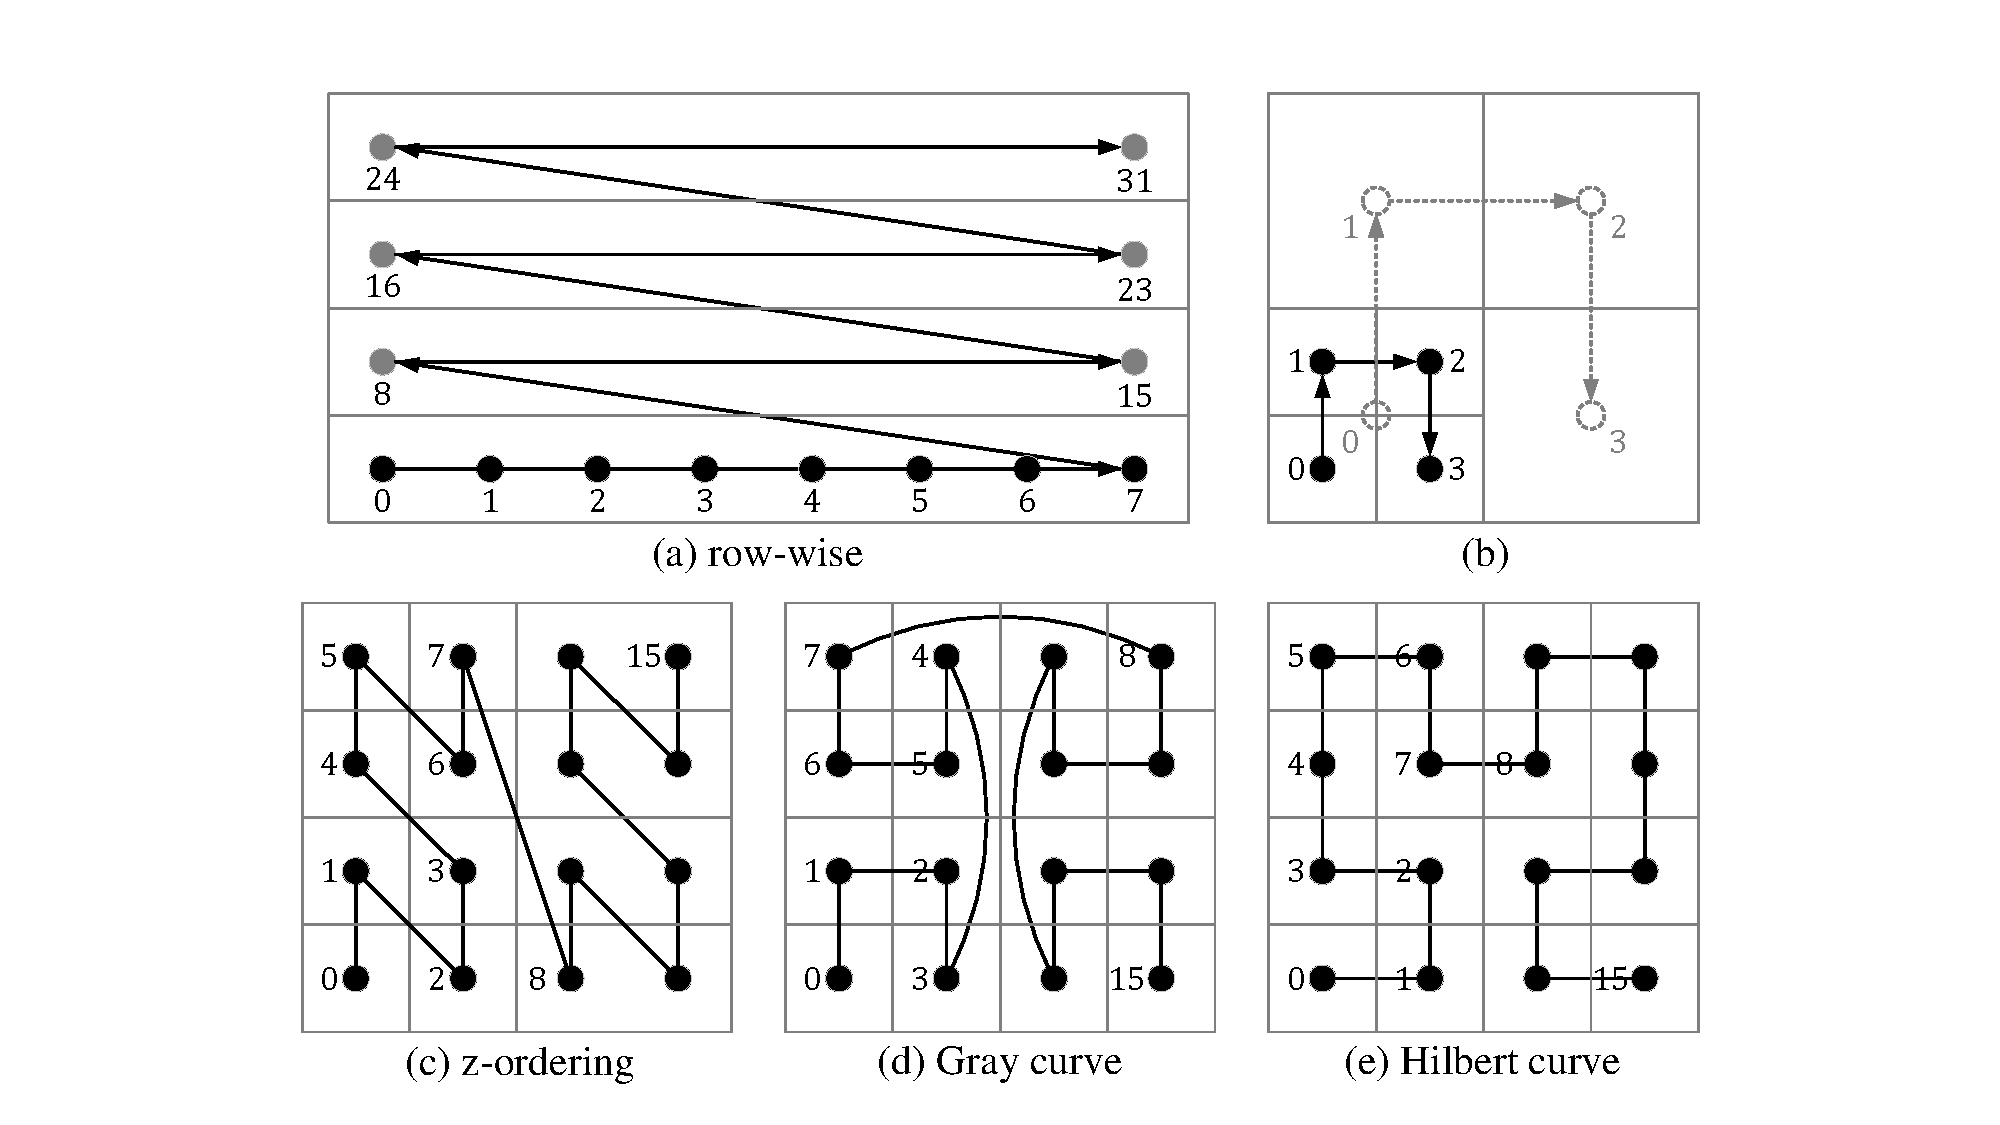
\includegraphics[width=0.75\textwidth]{linear-order.pdf}\\
  \caption{Different kinds of space-filling curves}\label{fig:sfc}
\end{figure*}

% 【sorting-keys的框架及其效果】
In the sorting-keys strategy, SK-LSH chooses to rearrange the compound hash keys under the row-wise curve to optimize the local distribution of candidates, because the compound LSH keys can well preserve the similarity among original data points. As a result, neighboring candidates are stored on the same or adjacent disk pages. It then defines a distance measure between compound hash keys to estimate the true distance between data points. During ANN search, a limited number of pages on the disk, which are ``close" to the query in terms of the distance defined between compound hash keys, are needed to be accessed for sufficient candidate generation, leading to much shorter response time due to the reduction of random I/O operations, yet with higher search accuracy.


\section{Overview of our method}\label{sec:overview}
In this section, we give deep explanations of the two major technical contributions in SC-LSH, the seeking for better linear orders and the reason we employ compact binary codes.

\subsection{Sorting keys under better linear order}\label{subsec:linearorder}
% sorting-keys作为基本框架
We take the sorting-keys strategy as the basic infrastructure of SC-LSH because it does help to improve the I/O performance, including both the I/O amount reduction and the I/O manner improving.
% 线序的选择有待商榷
However, as for the choice of linear order, we find that there are different kinds of space linear orders with different properties, and these properties have different effects on the local distribution of candidates.

\subsubsection{Mechanisms of space-filling curves}
% 曲线分类
Generally speaking, we can divide the space-filling curves into two categories according to their differences in setting the priority of space filling, the \emph{``dimension-first-traverse"} curve (short for DFT) and the \emph{``neighbor-first-traverse"} curve (short for NFT). Fig. \ref{fig:sfc} lists several samples of them. 
%For ease of expression, we shall use DFT and NFT to represent these two category respectively in the following content. 

Fig. \ref{fig:sfc}(a) depicts a kind of DFT curve, the row-wise curve, which is the curve employed in SK-LSH. Fig. \ref{fig:sfc}(c)(d)(e) depicts three kinds of curves, the z-ordering, the Gray curve and the Hilbert curve, respectively.

We can see clearly the differences on the priority they set for which to first traverse between these two categories of curves. For the row-wise curve, it specifies different priorities among different dimensions and will first traverse dimensions with higher priorities. Only when it goes through all the grids along the higher priority dimension, will it turn to the sub high-priority dimension to shift one step forward. After that, it turns back to the higher priority dimension and continues the filling. Suppose $(x, y)$ denotes the coordinate of a two-dimensional grid, and the X dimension has higher priority than the Y dimension. Its order on the curve will be $(y \cdot dim + x)$, where $dim$ represents the total number of coordinates along the X dimension.

NFT curves will first fill up a small local space, after that, they expand to a larger neighbor area and continue the filling. Usually, it exhibits an obvious recursion trend of a pre-defined filling logic during the expansion. Taking the Gray curve in Fig. \ref{fig:sfc}(d) as an example, the filling order conducted in the lower left 2$\times$2 grids is also the order to fill up the larger space when zooming in the whole 4$\times$4 grids as a bigger 2$\times$2 grids space as shown in Fig. \ref{fig:sfc}(b). Similar trends are also exhibited in the other two curves in Fig. \ref{fig:sfc}(c) and Fig. \ref{fig:sfc}(e).

\subsubsection{Better linear order}\label{sssec:anaorder}
% SK的做法,直观上认为不是最好的选择,好的线序,直观认为
Different mechanisms of space linear order could have different effects on the distribution of the candidates. SK-LSH does not conduct further study on that and chooses the row-wise curve as the order for keys sorting, which in our opinion is not the best choice. Better linear order should be able to better optimize the local distribution of NN candidates so that the candidates can be loaded in fewer I/O operations during the NN search. It is intuitively that the NFT orders could produce better NN candidates distribution than the DFT ones since NFT orders are more in line with the principle of nearest neighbor seeking for the nearest neighbors are usually distributed around the query point.
\begin{figure}[t]
	\centering
	% Requires \usepackage{graphicx}
	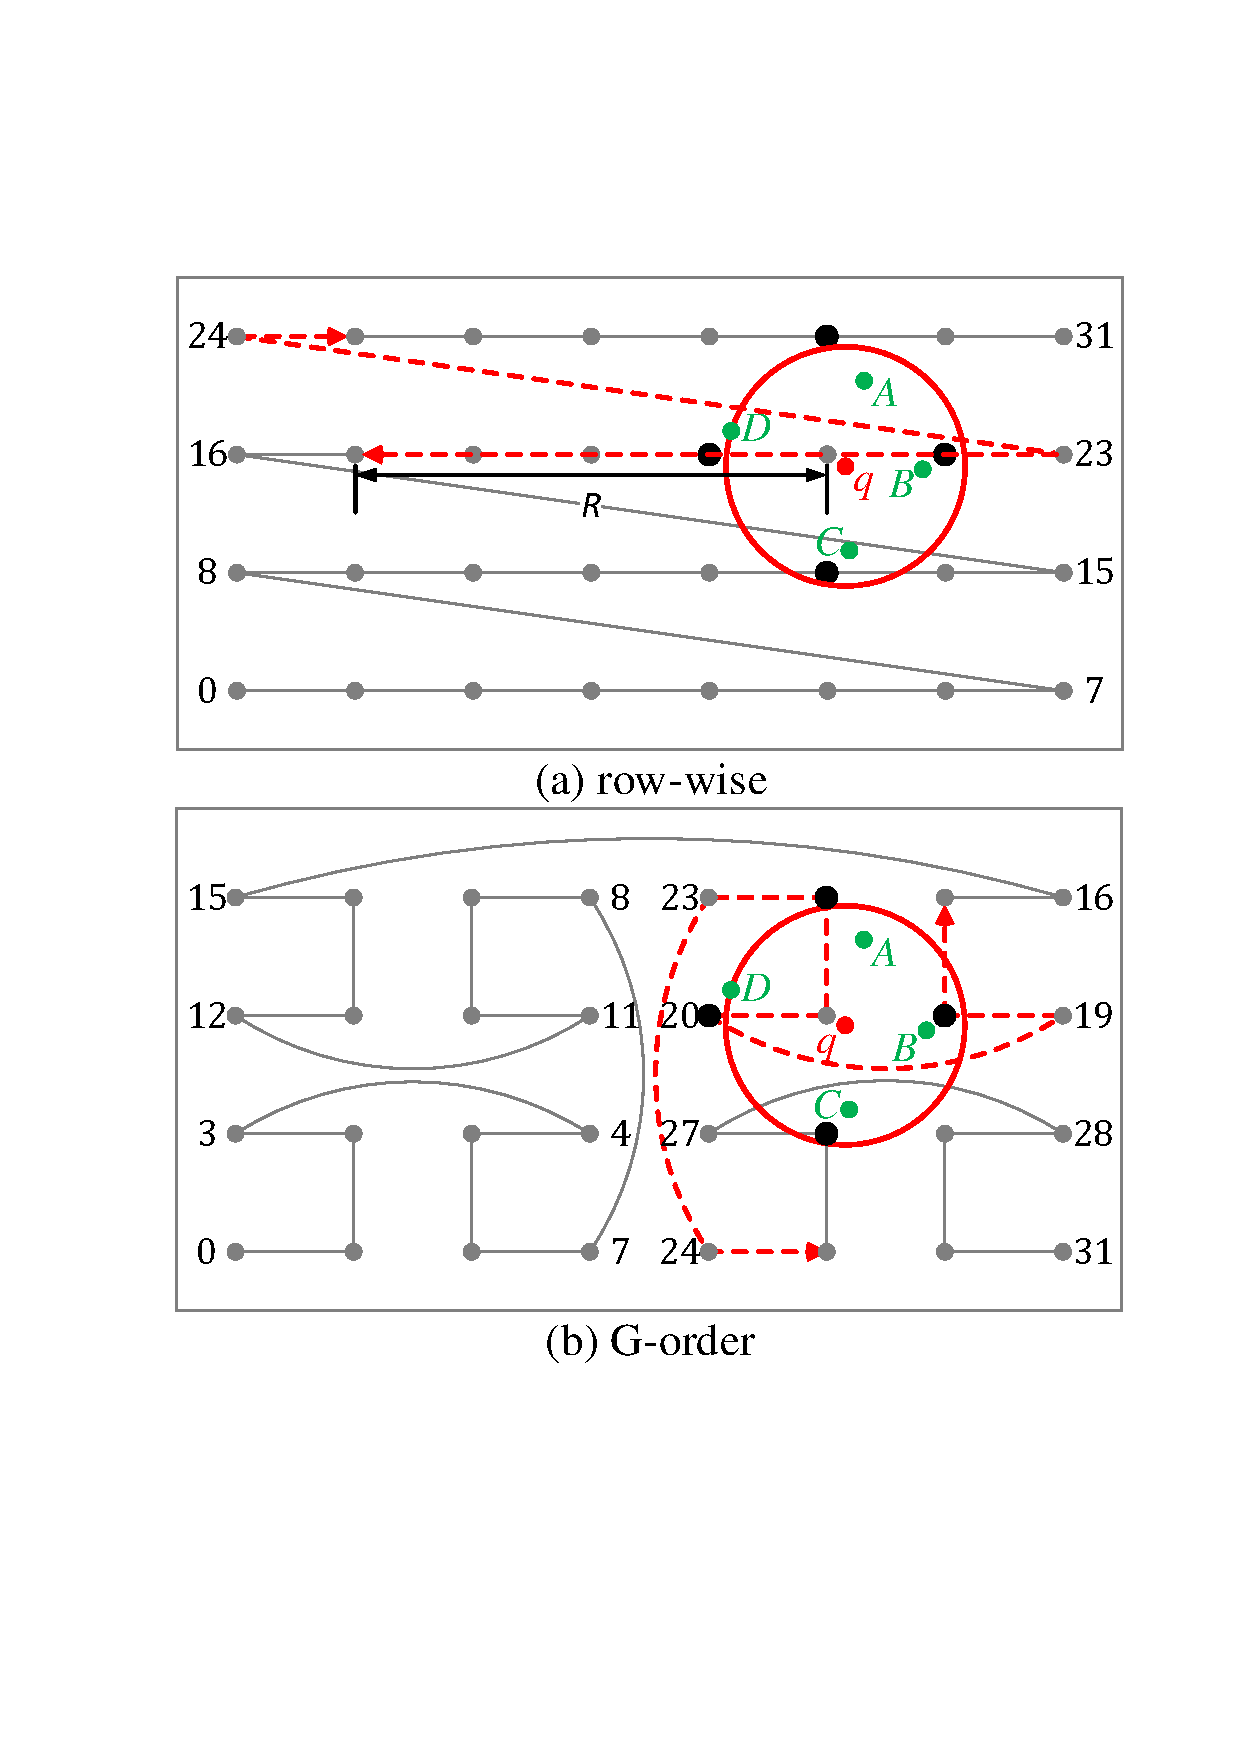
\includegraphics[width=0.45\textwidth]{order-compare.pdf}\\
	\caption{NN search test along two kinds of linear orders}\label{fig:nncompare}
\end{figure}

% 设置实验支撑观点
To verify our judgment, we conduct a series of quantitative experiments.
% 数据集生成:配置
We generate a set of synthetic datasets whose cardinality are fixed at 200,000 and the dimensionality vary in $\{2,4,8,12,16\}$ (that can cover the dimensionality we need to conduct the linear order in our method in the following parts). For each dataset, the coordinates are randomly generated following a uniform distribution under the range of [0, $S$], $S$ can be seen as the scale of the coordinates in each dimension. In our generation, we set $S=1,024$ for ease of parameter controlling. 


% 线序部署、数据存放、查询
For each dataset, we first split the whole space into equal-sized grids of width $W$. Then a certain kind of space-filling curve is conducted on all the grids. In this way, each data point can get its order alongside the curve according to the grid it locates in. We store all the data points on the disk according to their linear orders. 
% NN搜索:q, R, bidirectional, recall
When a query $q$ arrives, we first specify a search range $R$. Then we start a bidirectional search from the grids where $q$ locates in and load at most $R$ grids respectively in each direction. We count how many true $k$-NNs of $q$ can be found in the loaded data points. The recall rate $recall@k$ of the true $k$-NNs is used to judge the quality of the NN candidates distribution under a certain linear order.


% 举例说明:图,2维,网格划分,线序
To make a clear illustration, we take the NN search case in Fig. \ref{fig:nncompare} as an example. Fig. \ref{fig:nncompare} depicts two NN search cases in the 2-dimensional space. The grid width $W$ is set as 128, therefore, each dimension we can divide at most $n_I=S/W=8$ intervals (the edge of grid) as shown. We conduct two linear orders (the row-wise curve and the Gray curve) respectively to represent the two categories of linear orders. 
% q, true NN, k
Suppose $q$ is the query point, $\{A, B, C, D\}$ are its true 4-NNs. We set the search range $R=n_I/2$ which means $R=4$. Therefore all the grids that can be loaded will be determined (i.e., all the grids traversed by the red dotted lines in Fig. \ref{fig:nncompare}). As can be seen, on the row-wise order, we can get 2 true NNs, $\{B, D\}$, therefore the recall $recall_{row}@4=50\%$. As for the Gray curve, we will get three true NNs, $\{A, B, D\}$, the recall rate $recall_{Gray}@4=75\%$.

% 进一步地实验:比较两类线序,选择三个曲线来代表
Similar to the above settings, we conduct the NN search comparison between the DFT orders and the NFT orders on the generated datasets. We choose the row-wise curve from the DFT category and the Gray curve as well as the z-order curve from the NFT category. 
% 两类实验:参数,d, W, R
Two parameters are tuned respectively to conduct different comparisons, one is the dimensionality $d$, as shown in Fig. \ref{fig:order_compare_d}, the other is the grid width $W$, as shown in Fig. \ref{fig:order_compare_w}.   As for the recall target, we set $k=100$ to investigate the recall rate of the query's true 100-NNs.
% 详细的介绍R的计算,有些重复:We fix the search range $R=n_I/2$, here $n_I=S/W$ denotes the number of intervals divided along each dimension. Therefore, for a certain grid width $W$, we can figure out the corresponding search range $R=n_I/2=\frac{S}{2W}$.


%% 实验结果:row-wise对d和W很敏感
All the comparison results are listed in Fig. \ref{fig:order_compare_quan}. As shown, it is obvious that the row-wise curve is more sensitive to both the data dimensionality $d$ and the grid width $W$ than the other two curves.
\begin{figure*}[t]
	\begin{center}
		\subfigure[$recall$ versus $d$]{
			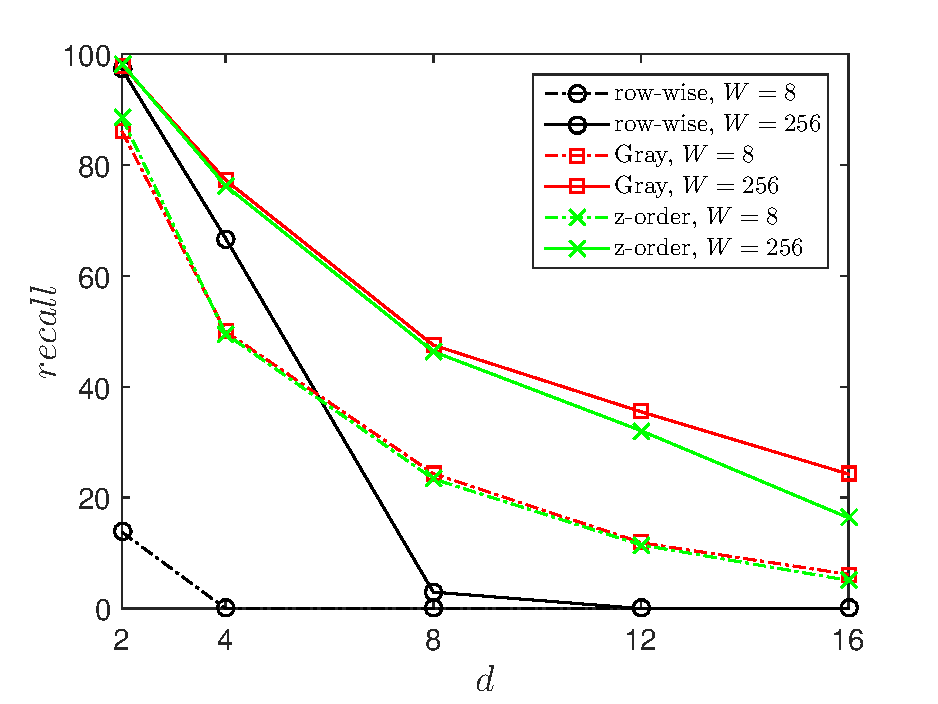
\includegraphics[width=0.45\textwidth]{order_compare_d.pdf} \label{fig:order_compare_d}
		}
		\subfigure[$recall$ versus $W$]{
			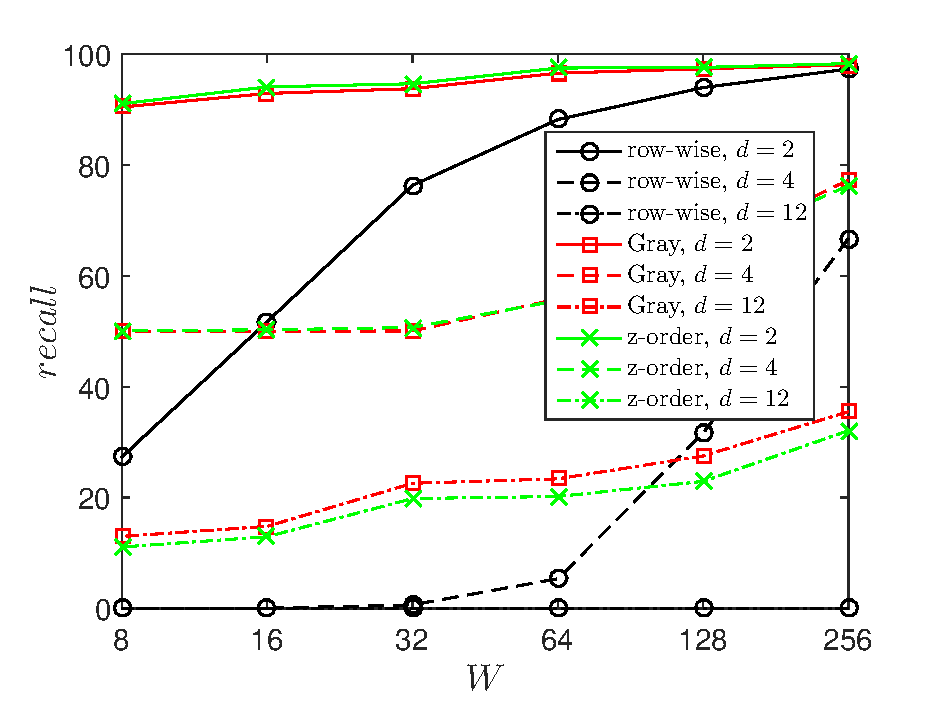
\includegraphics[width=0.45\textwidth]{order_compare_w.pdf} \label{fig:order_compare_w}
		}
	\end{center}
	\caption{Linear order comparison on synthetic datasets}\label{fig:order_compare_quan}
\end{figure*}

% 相对于d的效果:下降迅速,超过8,原因,分析
In Fig. \ref{fig:order_compare_d}, the recall rate on the row-wise curve exhibits a sharper decreasing trend with the growth of $d$. When $d$ is larger than 8, the NN search recall in both grid widths are nearly 0. This indicates that the row-wise curve is very easy to loss nearest neighbors in higher dimensions. This is caused by its dimension-first-traverse property, which is also the reason why point $A, C$ are missed in Fig. \ref{fig:nncompare}: because $A$ and $C$ are not located on higher priority dimension of the row-wise curve, they have to wait for one complete traverse along the other dimension before being accessed. And since most dimensions are of relatively lower priority, this could be more often when the dimension increases.
% 邻域优先遍历曲线
As for the other two curves, the neighbor-first-traverse property enables them traverse more NN candidates earlier in the local neighborhood than the DFT ones which makes them bear less influence from the data dimensionality. Although we cannot conduct linear orders on arbitrary high dimensions according to Fig. \ref{fig:order_compare_d}, for the dimensionality we need in our method (around 10-20), the NN distribution quality is good enough to support effective ANN search coupled with dimension reduction techniques with LSH.

% 相对于W的效果
We also set the linear order comparison versus different $W$ because we hear that SK-LSH is somewhat sensitive to the internal width $W$. If that is true, it may become another flaw of SK-LSH which could degrade the robustness of the ANN search algorithm. To verify that, we vary the grid width $W$ in a relatively wide range, from the relatively small width $W=8$ to a relatively large width $W=256$ (note that the scale $S$ of each dimension is at most 1,024) as shown in Fig. \ref{fig:order_compare_w}. Given a certain grid width $W$, the search range can be determined as $R=n_I/2=\frac{S}{2W}$.

% 实验结果
The result confirms our judgment. As can be seen in Fig. \ref{fig:order_compare_w}, when the width narrows, the recalls on all three curves exhibit decreasing trend. On the same dimension, the row-wise curve owns the most significant decreasing trend among them three. Again, this is caused by the characteristic of the curve, because the dimension-first-traverse property leads the row-wise curve to capture only a limited part of the real neighbors in the local neighborhood, much of the rest are missed. To ensure the query accuracy, one can enlarge the interval width so as to \emph{catch} those missed neighbors \emph{back} earlier. That is the reason why SK-LSH prefers to larger internal widths. However, the question is, enlarging the interval width $W$ will increase the collision probability of two distant points according to Equation \ref{eq:p(r,w)}, which means more false positives will be introduced into the candidate set and thus reduce the query accuracy. To make up of that, more LSH functions have to built to filter out these false positives adequately, which ultimately increases the index size as well as the computation overhead.

% NFT曲线
As for the NFT curves, they look not so sensitive to the change of $W$ as shown in Fig. \ref{fig:order_compare_w}. Although they also exhibit increasing trend with the help of enlarging $W$, they are not very dependent on it since they can produce relatively good recall of nearest neighbors even on narrow internals. 

%% 结论,线序的选择
In conclusion, different kinds of space-filling curves do have different effects on the local rearrangement of NN candidates, and the NFT curves perform better than DFT curves. This means NFT curves can help to further reduce the amount of I/O operations during the ANN search. Therefore, we will choose a kind of NFT curve for compound hash keys sorting in the following construction of SC-LSH.

% 我们的决定,选择
As for the choice, we possibly have three options, the z-ordering, the Gray curve and the Hilbert curve. Actually, the Hilbert curve can achieve the best clustering property to preserve the locality of data points among them three as reported in~\cite{Faloutsos1989Fractals}, however, it is a pity that the Hilbert curve is somewhat difficult to implement in the dimensions of the compound hash keys we need in SC-LSH. The Gray curve performs better NN distribution than the z-ordering curve as indicated in Fig. \ref{fig:order_compare_quan} and is as easy to implement as the z-ordering. Therefore, we finally choose the Gray curve. 
% Performs better than the z-ordering according to \cite{Faloutsos1989Fractals}.


\subsection{Candidate refining with compact binary codes}
\label{ssec:introPQ}
\subsubsection{Limitations of maintaining original data}\label{sssec:originallimitations}
% 原始数据维护带来的问题
Most LSH-based variants need to maintain one or more, sometimes hundreds or thousands, copies of original data points due to the need of discriminating real NNs from the candidate set in the refining phase. However, this sometimes becomes another typical limitation of LSH based methods, which concretely speaking, mainly resides in two aspects.
\begin{description}
  \item[$\bullet$] \textbf{Expensive space consumption} The space complexity of one copy of the original data points is $O(nd)$, for large scale high-dimensional dataset, this is very expensive and sometimes becomes the major space consumption of the index.
  \item[$\bullet$] % 去掉了SK-LSH的举例
    \textbf{Degrading the I/O scalability} The maintenance of original data points will degrade the I/O scalability in terms of dimensionality of some methods devoting for I/O efficiency improving. Suppose that a dataset $\textbf{D}\subset R^d$ resides in the external memory where each page occupies $B$ \emph{word}s. Then each page can hold nearly $B/d$ data points. To guarantee the ANN search accuracy, we often need to load sufficient candidate points. Without loss of generality, suppose that we load $\gamma$ points for each query, then the total number of disk pages we need to access is nearly $N_P=\gamma d/B=O(d)$ since $\gamma$ and $B$ can be seen as constants, which means the I/O cost is linearly proportional to the dimensionality. That is a poor scalability for external indexings.
\end{description}

% 对维护原始点提出疑问
The question is, do we necessarily have to keep the original data points in the index structure? The answer resides in the usage of them. We keep real data points because they can provide us with accurate distances between the candidates points and the query, and these distances can provide us with references to judge the quality the candidates so as to find out the real nearest neighbors.
%It is natural that the more accurate the distance is, the more precise nearest neighbors we get.
Hence, in fact, the actual point we care about is not the original distance value, but the ability of discriminating nearest neighbors. In other words, if we can find a space efficient way that can also preserve the similarity among real data points, we can avoid storing the original data and thus address the above limitations. Fortunately, the compact binary coding techniques can fulfill both the above requirements.

\subsubsection{Effect of compact binary codes}\label{ssec:compact}
% 紧凑编码技术的发展概述,代表技术
In recent years, the computer vision community has witnessed rapid progress in learning similarity-preserving binary codes to encode high-dimensional data points into compact binary codes~\cite{Gong2011,Torralba2008,Weiss08}. These codes could bring large efficiency gains in storage while preserving the similarity among the original data points. The most promising work resides in the research of product quantization (PQ)-based approaches~\cite{Jegou2011PQ,Babenko2012Inverted,Norouzi2013,WangWSXSL15,Yannis2014LOPQ}.

% including the original product quantization ~\cite{Jegou2011}, the product quantization with inverted multi-index ~\cite{Babenko2012Inverted}, the Cartesian K-Means (CK-Means) ~\cite{Norouzi2013} and the Optimized Cartesian K-Means method ~\cite{WangWSXSL15}. \cite{Yannis2014LOPQ}

%% PQ的原理
% 对量化中心的需要,原始VQ无法满足
As a quantization technique, PQ is derived from vector quantization (VQ), which reduces the representation space to a codebook $\textbf{C}$ composed of $\mathbb{K}$ codewords (or centroids) $\{c_i\}_{=1}^\mathbb{K}$ generated from clustering algorithms. A data point $p\in \textbf{D}$ is mapped into its nearest centroid under the Lloyd optimality conditions in terms of Euclidean distance:
\begin{equation}
\label{eq:vqmap}
\pi \left( p \right) = \mathop {\arg \min }\limits_{{c_i} \in \textbf{C}} \left\| {p,{c_i}} \right\|_2
\end{equation}
Here, $\pi(\cdot)$ is the quantizer, $\left\|,\right\|_2$ indicates the Euclidean distance and the index $i$ can be seen as the quantized code of $p$. For any two points $p_i,p_j\in \textbf{D}$, their distance can be estimated according to the quantized codes, i.e., $\left\|{p_i,p_j}\right\|_2 \approx \left\|{\pi(p_i),\pi(p_j)}\right\|_2$. For vector quantization, to obtain precise estimated distances, the quantization error must be limited. Therefore, the total number $\mathcal{K}$ of centroids should be sufficiently large. However, for typical vector quantization techniques, such as K-Means and hierarchical K-Means (HKM), one issue is the scalability of codebook. It is hard for them to scale to large $\mathcal{K}$ (e.g. $\mathcal{K}=2^{64}$) since both the codebook storage and data point assignments become untenable.

% PQ的做法
PQ successfully addresses this issue with a model of compositional parameterization of cluster centroids. Suppose that $d$ is a multiple of $\mathcal{M}$ and $\mathcal{S}=d/\mathcal{M}$. In PQ-based methods, the data space is firstly decomposed into a Cartesian product of $\mathcal{M}$ $\mathcal{S}$-dimensional subspaces, and each vector $p\in \textbf{D}$ can be seen as a concatenation of $\mathcal{M}$ disjoint $\mathcal{S}$-dimensional sub vectors $u_j(p)$, $1\le j \le \mathcal{M}$:
$$
p = \underbrace {{p^1}, \cdots ,{p^\mathcal{S}}}_{{u_1}\left( p \right)}, \cdots ,\underbrace {{p^{d - \mathcal{S} + 1}}, \cdots ,{p^d}}_{{u_{M}\left( p \right)}}
$$
Then, K-Means is performed to obtain a sub codebook containing $k^*$ sub codewords in each subspace. By this means, a codebook $\textbf{C}$ containing ${k^*}^\mathcal{M}$ centroids is generated using the Cartesian product of these sub codebooks:
$$
\textbf{C}=\textbf{C}_1 \times \cdots \times \textbf{C}_{\mathcal{M}}
$$
Note that the storage of the codebook $\textbf{C}$ is only $O(k^* d)$, while K-Means requires $O({k^*}^\mathcal{M}d)$ storage with the same number of centroids. Using these sub codebooks, a data point $p$ can be mapped as follows:
$$
\begin{array}{*{20}{l}}
{p \to \pi \left( p \right)}& = &{\left( {{\pi _1}\left( {{u_1}\left( p \right)} \right), \ldots ,{\pi _\mathcal{M}}\left( {{u_\mathcal{M}}\left( p \right)} \right)} \right)}\\
{}& = &{\left( {{\textbf{C}_1}[{i_1}], \ldots ,{\textbf{C}_\mathcal{M}}[{i_\mathcal{M}}]} \right)}
\end{array}
$$
Here, $\pi_j(\cdot)$ is the subquantizer in the $j$-th subspace. By concatenating the indexes of the $\mathcal{M}$ centroids returned by the $\mathcal{M}$ subquantizers, we can encode the data point $p$ into a compact PQ code:
$$
Q\left( p \right) = \left( {{i_1}, \ldots ,{i_M}} \right)
$$
Note that the time complexity of the data point encoding is reduced from $O({k^*}^\mathcal{M}d)$ in K-Means to $O(k^* d)$ here. Besides, $k^*$ is usually set to be a power of 2. Let $\mathcal{U}=\log_2k^*$, each PQ code is thus a $\mathcal{UM}$-bit binary string which will occupy $s=\mathcal{UM}/32$ machine words in total.

% 距离计算方式
In addition to the high estimation precision, PQ conducts a kind of \emph{asymmetric quantizer distance (AQD)} to estimate the square distance between a data point $p$ and the query vector $q$ without quantizing $q$:
\begin{equation}
\label{eq:aqd}
\left\| {q,p} \right\|_2^2 \approx \left\| {q,\pi \left( p \right)} \right\|_2^2 = \sum\limits_{j = 1}^\mathcal{M} {\left\| {{u_j}\left( q \right),{C_j}\left[ {{i_j}} \right]} \right\|_2^2}
\end{equation}
This can be done efficiently with the help of a pre-computed lookup table. According to Equation \ref{eq:aqd}, by pre-computing all the square distances between each sub query vectors $u_j(q)$ and the sub codewords in the $j$-th sub codebook $\textbf{C}_j$, the AQD square distance computation between $p$ and $q$ is transformed into a table lookuping with the PQ code components in $Q(p)$ as the indexes. Inspired by \cite{andre2015cachePQ}, we depict this procedure vividly in Figure \ref{fig:lookup}, where we generate 64-bit PQ codes with $\mathcal{M}=8$ and $k^*=256$.
\begin{figure}[t]
\begin{center}
{
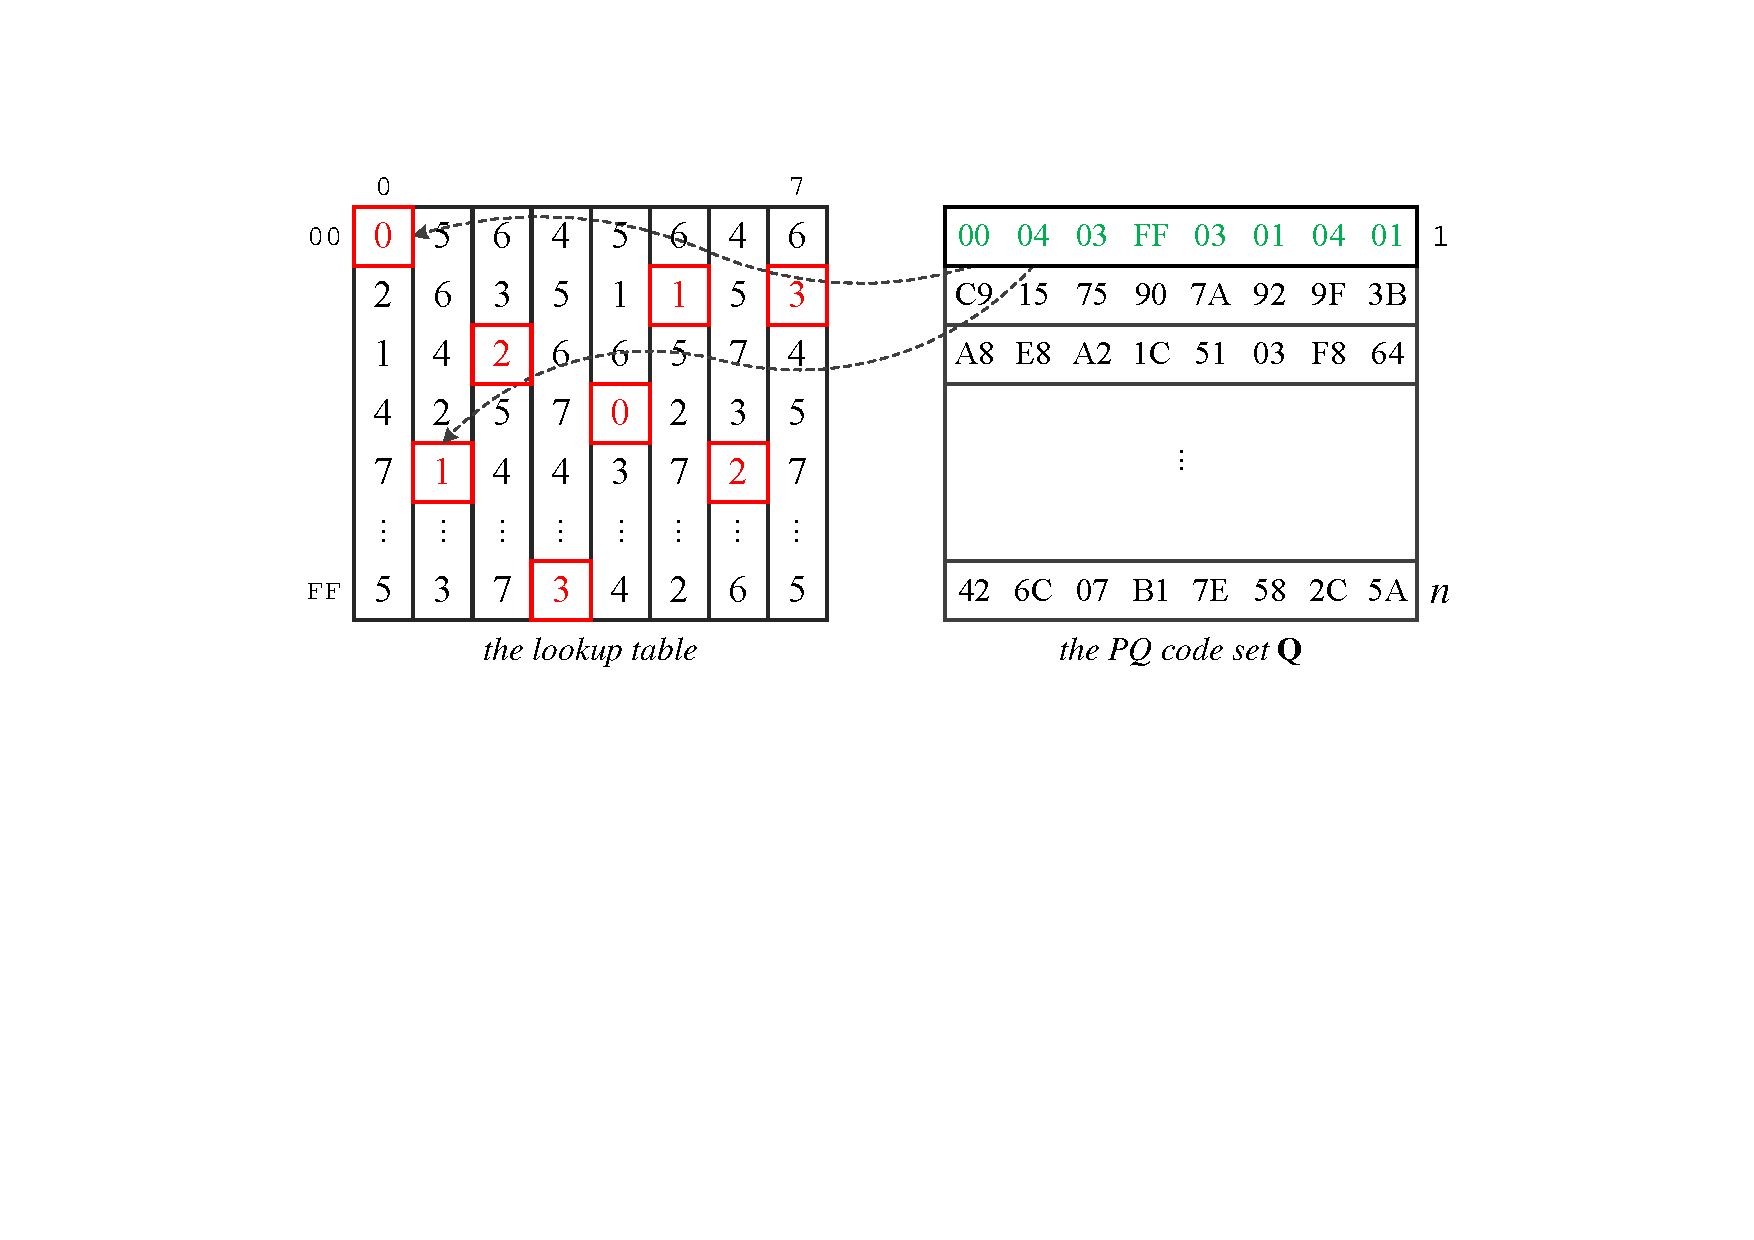
\includegraphics[width=0.49\textwidth]{lookup.pdf}
}
\end{center}
\caption{Illustration of distance estimation using a lookup table}
\label{fig:lookup}
\end{figure}

% 介绍使用了紧凑编码后的效果
Since the compact binary codes, especially the PQ series are very space efficient and are accurate enough to discriminate nearest neighbors due to their high quantization accuracy, we decide to store compact binary codes instead of the original data points to do candidates refining in SC-LSH.
% 具体使用的编码
More specifically, we focus on product quantizers with $2^{64}$ centroids, which means each PQ code occupies 64-bit storage. According to the performance estimation conducted in \cite{Jegou2011PQ} and \cite{Norouzi2013}, the 64-bit long codes are good enough to produce sufficiently high quantization accuracy for most typical high-dimensional datasets, especially for the datasets chosen in our experiments in Section \ref{sec:er}. 64 bits means 2 words. This constant storage means a compression ratio of $d/2$ (suppose that each component of the data point is a one word long integer/float) of the storage of the original data set. Besides, it also means that one disk page ($B$ words) now can hold $B/2$ data codes, not only gets rid of the limitation from the dimensionality $d$, but also be enlarged to a big constant. Therefore, a few page accesses are much enough to load sufficient candidates. Both the two limitations caused by maintaining original data points (mentioned at the beginning of this section) will be eliminated.

\section{SC-LSH}\label{sec:sclsh}
In this section, we introduce all necessary details to apply SC-LSH to address ANN search, including the linear order deploying, the indexing construction and the ANN search algorithm.

\subsection{G-order over compound hash keys}\label{ssec:linearorder}
We choose the Gray curve as the linear order (denoted as G-order) conducted over the compound hash keys in SC-LSH. We firstly make some necessary definitions.

\begin{definition}
\label{def:g-order}
(\textbf{G value}) The Gray curve projects the data in the $I^m$ space to an integer in $I$, denoted as $G:I^m\rightarrow I$. For a data point $o\in \textbf{D} \subset R^d$, let $K=\{k_i\}_{=1}^m=\mathcal{G}(o), k_i \in I$ denotes the compound hash key of $o$ under a compound hash function $\mathcal{G}$ which consists of $m$ LSH functions. $G(o)$ is called the \emph{G value} of $o$. According to \cite{Faloutsos1989Fractals}, the computing of G value mainly consists of three steps, all of which are easy to implement.
\end{definition}

% 对m维复合哈希键值的编码过程
% For any data point $o\in \textbf{D} \subset R^d$, $K=\{k_i\}_{=1}^m=\mathcal{G}(o)$ denotes the compound hash key of $o$ under the compound hash function $\mathcal{G}$ which consists of $m$ LSH functions. We can compute the G value of $o$ under $\mathcal{G}$ as follows. Firstly, we represent each component $k_i$ of $K$ as a $u$-bit long binary string, then we interleave all the binary string following the method depicted in Fig. \ref{fig:zordering} and we will get a $um$-bit long binary string, the decimal value of this binary string is the Z value $Z(o)$ of point $o$.

\begin{definition}
\label{def:zprefix}
(\textbf{Prefix of G values }) Given a data point $o\in R^d$ and its G value $G(o)=g_1g_2\cdots g_S$ where $S=um$ is the length of the G value, let $l$ denote the length of the prefix, we define the prefix of the G value as:
\begin{equation}
\label{eq:zprefix}
pref(G,l)=(g_1g_2\cdots g_l)
\end{equation}
\end{definition}

\begin{definition}
\label{def:gncpl}
(\textbf{Length of the non-common prefix of G values}) Given two G values $G_1=(g_{1,1}g_{1,2}\cdots g_{1,S})$ and $G_2=(g_{2,1}g_{2,2}\cdots g_{2,S})$, if $pref(G_1,l)=pref(G_2,l)$ and $pref(G_1,l+1)\neq pref(G_2, l+1)$, then we can define the length of the non-common prefix between $G_1, G_2$ as:
\begin{equation}
\label{eq:gncpl}
NL(G_1,G_2)=S-l
\end{equation}
Specially, if $pref(G_1,S)=pref(G_2,S)$, we have $NL(G_1,G_2)=0$.
\end{definition}

\begin{definition}
\label{def:gdis}
(\textbf{Distance over G values}) For two data points $o_1, o_2 \in \textbf{D}$, we define the distance between their G values $G_1,G_2$ as follows:
\begin{equation}
\label{eq:gdis}
dist_G(G_1,G_2)=NL(G_1,G_2)
\end{equation}
\end{definition}

\begin{definition}
\label{def:gpartial}
(\textbf{Partial order over G values}) For two data points $o_1, o_2 \in \textbf{D}$, we define a partial order $\langle G, \leq_G \rangle$ for their G values $G_1,G_2$:
\begin{equation}\label{eq:gpartialorder}
\left\{ {\begin{array}{ll}
{G_1<_G G_2,} & {if\ l<S\ and\ g_{1,l+1}<g_{2,l+1}} \\
{G_1=_G G_2,} & {if\ l=S}\\
{G_2<_G G_1,} & {if\ l<S\ and\ g_{1,l+1}>g_{2,l+1}}
\end{array}} \right.
\end{equation}
here, $l=S-NL(G_1,G_2)$.
\end{definition}

\subsection{Indexing}\label{ssec:indexing}
In SC-LSH, all the data are deposited in $\mathcal{L}$ hash tables $\textbf{T}=\{T_i\}_{=1}^{\mathcal{L}}$, each hash table $T$ contains totally three kinds of data, 1) a G value set $\textbf{G}$ of the original data, 2) a PQ code set $\textbf{Q}$ of the original data and a sorted ID list $\textbf{ID}'$ of the original data points. There are several other kinds of data, including the original data points and the compound hash keys which we are certain to generate, however all of them will only appear in the intermediate process of the index building, we do not finally maintain them in the index structure.

Fig. \ref{fig:indexing} depicts the construction procedure of the index structure. Overall, it consists of three phases, the ordering phase, the sorting-codes phase and the tree-building phase.
\begin{figure}
  \centering
  % Requires \usepackage{graphicx}
  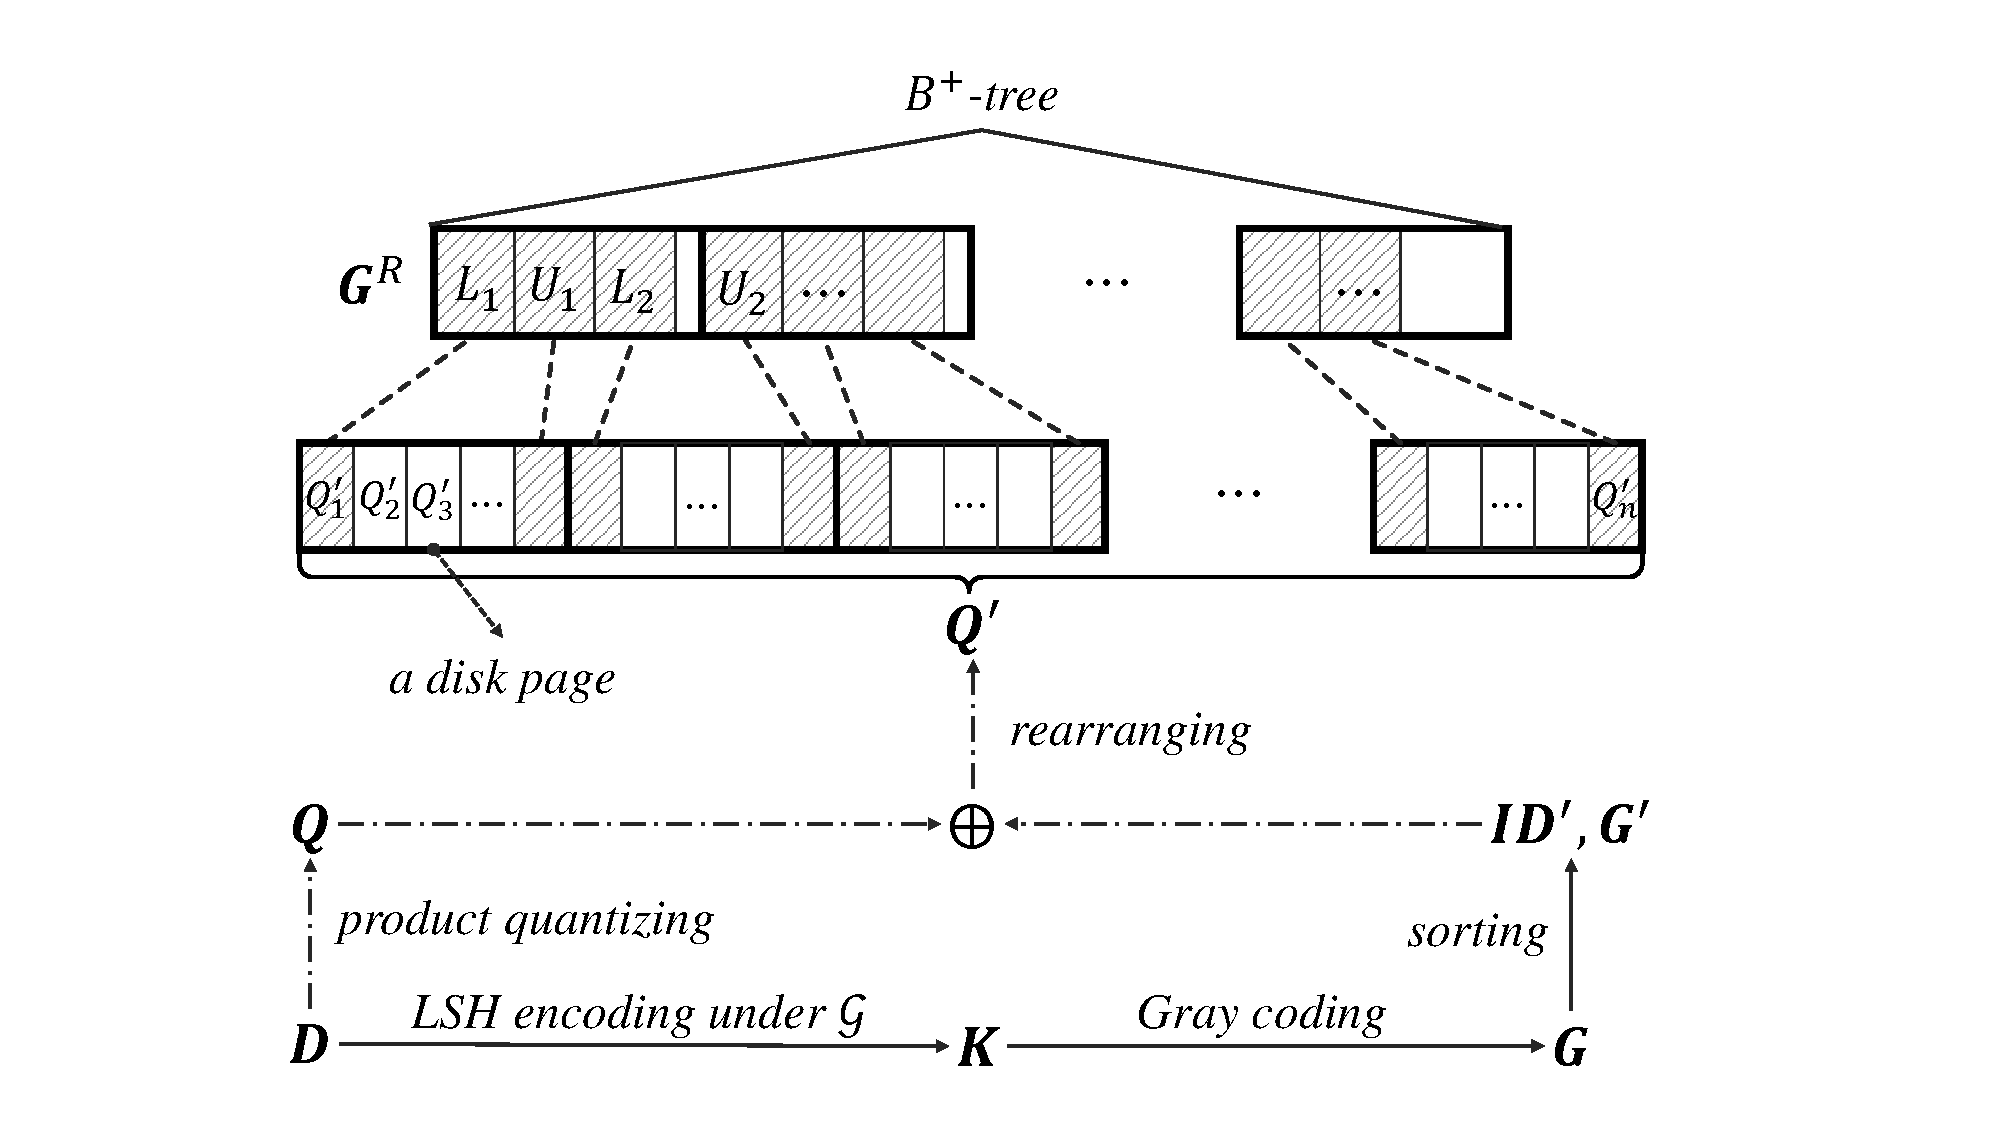
\includegraphics[width=0.45\textwidth]{indexing.pdf}\\
  \caption{Index construction}\label{fig:indexing}
\end{figure}

In the order phase, we firstly generate the compound hash key set $\textbf{K}$ for all data points in $\textbf{D}$ under a compound hash function $\mathcal{G}$. Then we convert them into G values and get the corresponding G value set $\textbf{G}$. Next, we sort all the G values in ascending order according to the linear order defined in Equation \ref{eq:gpartialorder} and get a sorted G value set $\textbf{G}'$ together with the sorted ID list $\textbf{ID}'$ of the original data points.
% 数据点ID的来历, note that the ID of a data point is just its sequence number in the original data set $\textbf{D}$ which is started from 0.

After we get the sorted G values, we come into the codes-sorting phase, in which we first generate the data codes $\textbf{Q}$ for all the original data points under a pre-defined product quantizer. Then we rearrange them according to the order in $\textbf{ID}'$ and get a sorted code set $\textbf{Q}'$. $\textbf{Q}'$ will finally be stored on the external memory. We specify $s$ measured in machine words to denote the size of one PQ code, then the capacity of a $B$ machine words disk page for PQ codes becomes:
\begin{equation}\label{eq:vq}
V=\lfloor B/s \rfloor
\end{equation}

The final phase is the tree-building. Different from SK-LSH, we maintain G values instead of compound hash keys in the B$^+$-trees. Note that, we do not maintain all the G values in $\textbf{G}$, we extract a representative G value set $\textbf{G}^R$ from it. Concretely, we represent each data page (full of PQ codes now) by extracting a pair of G values $\langle L, U \rangle$ which belong to the first and the last data code respectively on a certain disk page. Then a B$^+$-tree is built over all the representative G values pairs $\textbf{	G}^R$ as shown in Fig. \ref{fig:indexing}. Note that the total number of data pages storing PQ codes is $\lceil n/V \rceil$, then the total number of the representative G values becomes:
\begin{equation}\label{eq:nrepg}
R = 2\lceil n/V \rceil \approx 2ns/B
\end{equation}
This means a compression ratio of nearly ${B}/{(2s)}$ of G value storage. Besides, $s \ll B$ usually holds, for example, 64-bit PQ codes in 4KB disk pages means $s=2$ and $B=1024$. Therefore, it is a significant space saving for the index structure while not degrade the routing effect of the B$^+$-tree in ANN search.

In conclusion, during the entire process of index constructing, we use one set of product quantizer to generate PQ codes and $\mathcal{L}$ set of compound hash functions for LSH encoding. Therefore, the index structure of SC-LSH contains $\mathcal{L}$ B$^{+}$-trees, $\mathcal{L}$ set of ID permutations and $\mathcal{L}$ set of relatively sorted data codes.

\subsection{ANN Search}\label{subsec:annsearch}
% 算法的终止条件,决定磁盘页面需要加载顺序,从而引出查询点-页面距离定义
During the ANN search in SC-LSH, we set the termination condition as the number of data pages $N_P$ allowed to be accessed in order to make a better control of both the accuracy and the I/O efficiency. As a result, we need to carefully determine the order of page accessing to make sure that more data items with higher quality can be reached during the search process. To achieve that, we firstly define the distance between a query point and a data page as follows:
\begin{definition}
\label{def:distP}
(\textbf{Distance between a query point and a data page}) Given a query point $q$ and a data page $P_i$ containing at most $V$ data codes, let $G_q$ be the G value of $q$ and a pair of G values $\langle L_i, U_i \rangle$ to denote $P_i$. The distance between the query point $q$ and $P_i$, denoted as $dist_{Page}(q,P_i)$, is calculated as follows:
\begin{equation}
\label{eq:distP}
dist_{Page}(q,P_i) = \left\{ \begin{array}{ll}
dist_G(G_q, L_i) & \textrm{if $G_q \leq_G L_i$} \\
0 & \textrm{if $L_i \leq_G G_q \leq_G U_i$} \\
dist_G(G_q, U_i) & \textrm{if $U_i \leq_G G_q$}
\end{array} \right.
\end{equation}
\end{definition}

% 解释查询点到页面的距离的含义 - ###可加可不加
As shown in Definition \ref{def:distP}, for $G_q$ and $\langle L_i,U_i\rangle$, there are three cases which need to be considered. In the first case, $G_q$ is smaller than all the G values of the data items in $P_i$. So the lower bound of distances between $G_q$ and the G values of data items in $P_i$ is $dist_G(G_q, L_i)$. In the second case where $G_q$ falls into the range between $L_i$ and $U_i$, the distance of $G_q$ and page $P_i$ is defined as 0. In the third case where $G_q$ is greater than all G values of data items in $P_i$, the lower bound is $dist_G(G_q, U_i)$.

% 查询时定位到最近页面
Based on the above definition, we discuss in the following how to find the closest page to $q$ in a sorted code set. Let $n$ be the cardinality of $\textbf{D}$ and $\rho = \lceil n/V \rceil$ be the number of data code pages. In addition, we use $\textbf{P} = \{P_1, P_2, \dots, P_{\rho}\}$ to refer to the all the data code pages. Note that, a B$^+$-tree in the index structure is created to index all the representative G values $\Theta = \{L_1, U_1, L_2, U_2, \dots, L_{\rho}, U_{\rho}\}$. It is very convenient to find two G values in $\Theta$, $\theta_i$ and $\theta_{i+1}$ ($1 \leq i \leq 2\rho-1$), such that $\theta_i \leq G_q \leq \theta_{i+1}$ by searching in the B$^+$-tree. If $\lceil \frac{i}{2} \rceil = \lceil \frac{i+1}{2} \rceil$, indicating that $\theta_{i}$ and $\theta_{i+1}$ belong to the same data page $P_{\lceil \frac{i}{2} \rceil}$, the closest data page to $q$ is $P_{\lceil \frac{i}{2} \rceil}$ according to Definition \ref{def:distP}. Otherwise, $\theta_{i}$ and $\theta_{i+1}$ belong to different data pages and we compare the distances of $P_{\lceil \frac{i}{2} \rceil}$ and $P_{\lceil \frac{i+1}{2} \rceil}$ to $q$ respectively to figure out the closest one.

% 需要确定在多个哈希表间加载页面的方法
In SC-LSH, we employ $\mathcal{L}$ index files in order to reduce the loss of false negatives. The key operation for ANN search is to find the next data page to be accessed among $\mathcal{L}$ B$^+$-trees in the index files, which can be done by bi-directional expansion at data pages of all B$^+$-trees. Algorithm \ref{alg:mts} summarizes the whole search process in multiple hash tables of SC-LSH.
\begin{algorithm}[t]
\caption{$k$-ANN search on multi-trees}
\label{alg:mts}
\begin{algorithmic}[1]
\REQUIRE hash tables $\textbf{T}=\{T_{i}|1 \leq i \leq \mathcal{L}\}$, query point $q$, number of returned nearest neighbors $k$, termination condition $N_{P}$;
\ENSURE $k$ nearest neighbors $k$NN[];
\STATE Initialize $o$=NULL, page counter $cnt$=0;
\FOR{$i = 1$ to $\mathcal{L}$}
\STATE Compute the G values $G_{q}^i$ of $q$;
\STATE Find out the initial pages $P_{iL}$ and $P_{iR}$, push them into $\Phi$;
\ENDFOR
\REPEAT
\STATE $P = extract(\Phi)$;
\STATE Verify data codes on page $P$ to update $k$NN[], make sure $k$NN[] keeps the data items with the smallest $k$ AQD to $q$ up to now;
\STATE $cnt$++;
\STATE $P' = shift(P)$;
\STATE $\Phi = \Phi \cup P'$;
\UNTIL{$cnt \geq N_{p}$}
\RETURN $k$NN[];
\end{algorithmic}
\end{algorithm}

% 为每个页面初始化指针
Firstly, we set two pointers $P_{iL}$ and $P_{iR}$ on each hash table $T_i$ to help guide the page accessing, as shown in line 2-5 in Algorithm \ref{alg:mts} where $1\leq i \leq \mathcal{L}$. We use $P_{iL}$ to denote the closest data page to $q$ in $T_i$, and $P_{iR}$ to the data page immediately succeeding $P_{iL}$. Figure \ref{fig:search} shows an example where 3 index files are built.
% 举例说明过程
Taking $T_1$ as an example, $P_{12}$ has the smallest distance to $G_{q}^1$. Hence, $P_{1L}$ is set to be $P_{12}$ and $P_{13}$ as $P_{1R}$. Similarly, we obtain $P_{2L}$, $P_{2R}$, $P_{3L}$ and $P_{3R}$. It is easily derived that the page with the smallest distance to its corresponding G value of the query point must be in the set $\Phi=\{P_{1L}, P_{1R}, P_{2L}, P_{2R}, P_{3L}, P_{3R} \}$.

% 循环记载页面并验证
Line 6-12 in Algorithm \ref{alg:mts} describes the loop where we constantly determine the next data page to load and verify the candidates among $\mathcal{L}$ hash tables. To facilitate the discussion, we define two operations on $\Phi$, $extract$ and $shift$. $extract(\Phi)$ returns the closest data page in $\Phi$, say $P^*$, and $P^*$ is meanwhile removed from $\Phi$. $shift(P)$, where $P \in \Phi$, means moving the pointer to $P$ away from $q$ by one page to $P'$. For instance, the result of $shift(P_{1L})$ is $P_{11}$ and that of $shift(P_{2R})$ is $P_{24}$. Usually, we will use the new page $shift(P)$ to replace $P$ in $\Phi$ as shown in line 10-11. By repeating $extract$ and $shift$ operations, close data pages to the query point will be found from all B$^+$-trees in sequence.
% PQ的距离计算
Before we do candidate refining, we need to prepare a lookup table composed of the squared distances between each sub vector of the query point and each sub codewords. After we load the candidate PQ codes into the memory, we perform AQD computations between the codes and the query according to Equation \ref{eq:aqd} based on the lookup table to determining nearest neighbors (line 8).

% 终止
Finally, if the number of data pages verified exceeds a threshold, $N_P$, specified before the search, SC-LSH terminates the search process (line 12 in Algorithm \ref{alg:mts}). Additionally, we recommend to maintain a bitmap in the algorithm to avoid unnecessary replicated verification.
\begin{figure}[t]
	\begin{center}
		{
			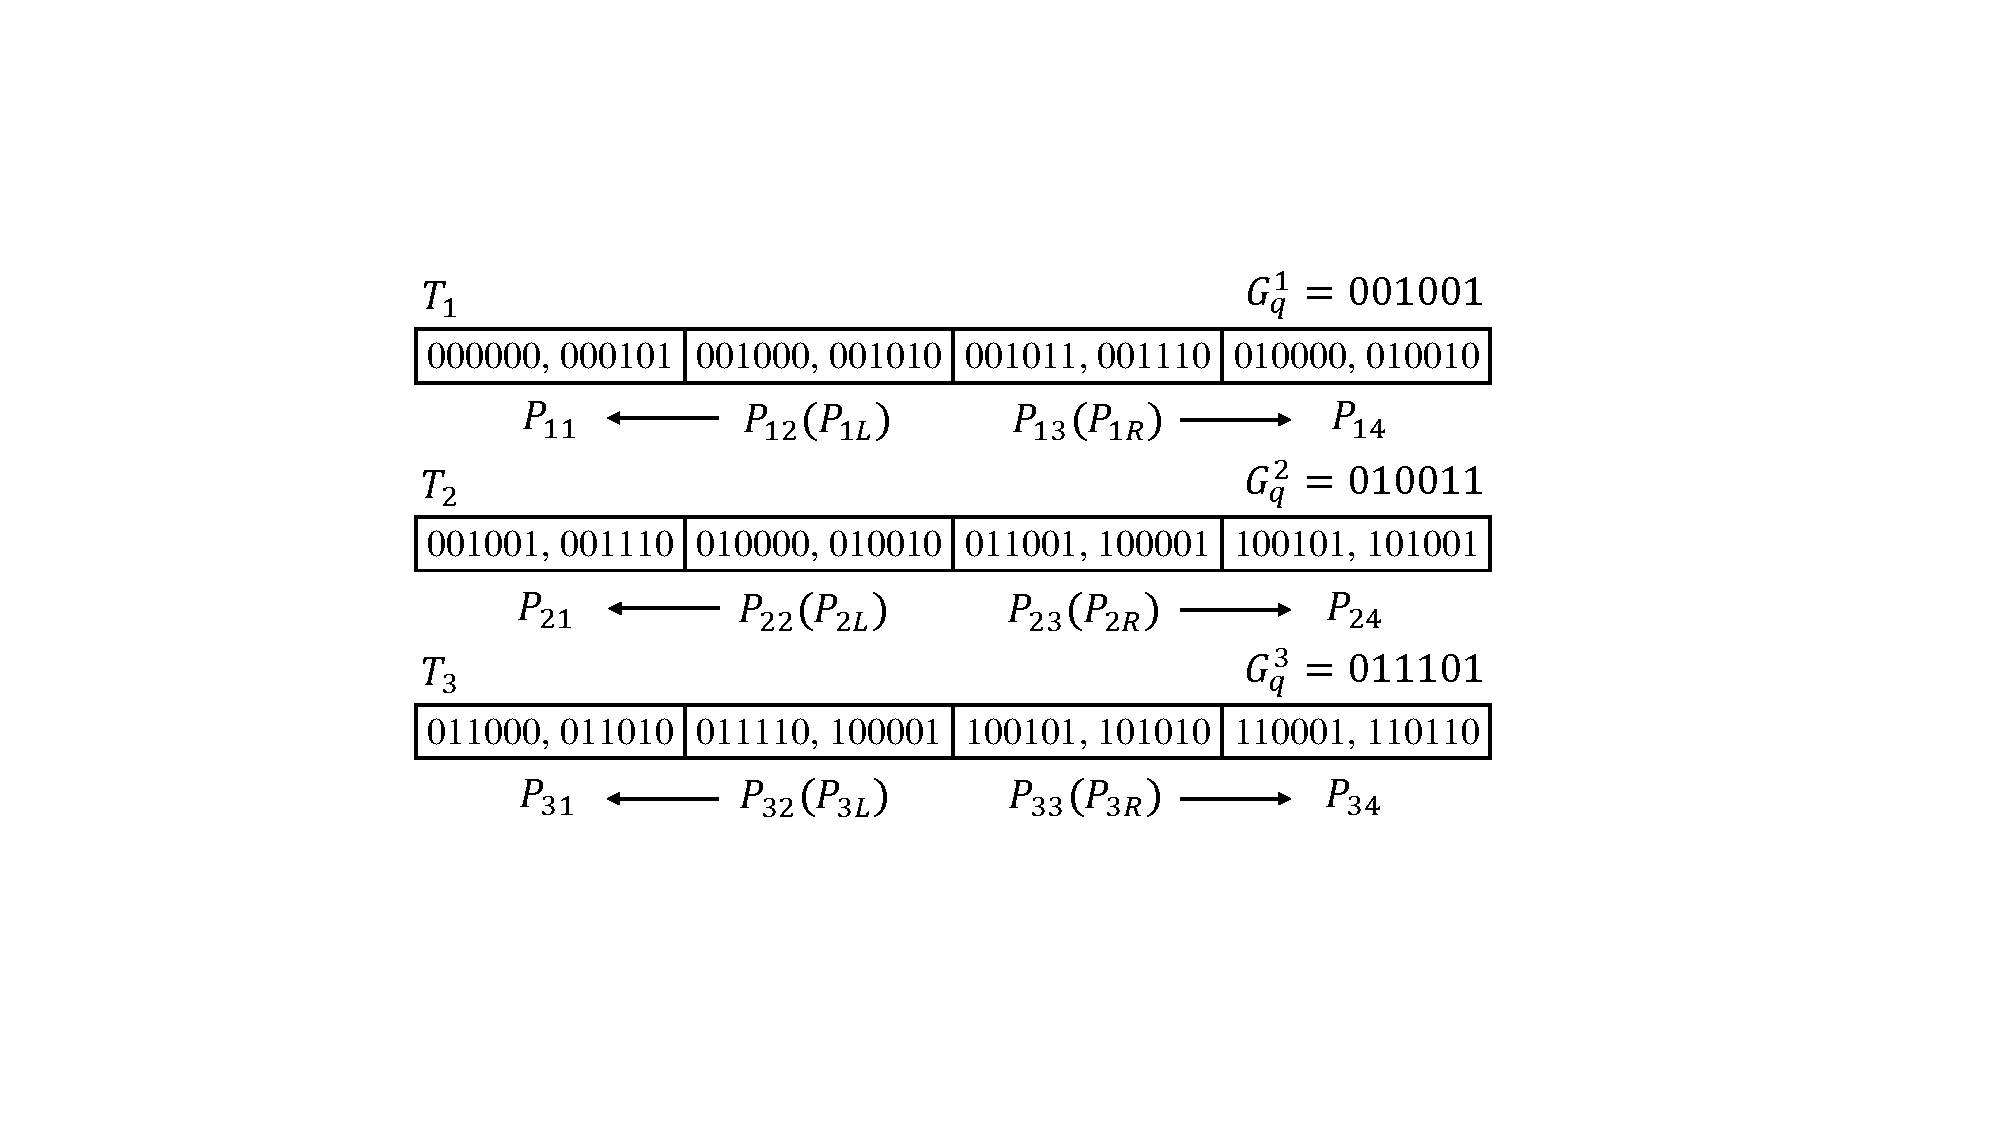
\includegraphics[width=0.48\textwidth]{search.pdf}
		}
	\end{center}
	\caption{Bi-directional expansion}
	\label{fig:search}
\end{figure}


\subsection{Complexity analysis}\label{ssec:complex}
% Space complexity
As mentioned in Section \ref{ssec:indexing}, the space consumption of SC-LSH mainly consists of three parts, 1) parameters of $\mathcal{L}$ set of compound hash functions, totally $\mathcal{L}md$, 2) $\mathcal{L}$ set of sorted ID list, totally $\mathcal{L}n$ and 3) $\mathcal{L}$ hash tables where each contains a B$^+$-tree maintaining a set of representative G values and one set of data codes. According to Equation \ref{eq:nrepg}, there are totally about $R =2ns/B$ representative G values to maintain in a B$^+$-tree. Therefore, the total space consumption of SC-LSH will be $O(\mathcal{L}(md+n+ns(2m/B+1))$. Usually $2m \ll B$ holds in practical cases, then the space consumption will become $O(\mathcal{L}(md+n(s+1)))$. Note that this is a remarkable progress compared with SK-LSH since we make the space consumption get rid of the limitation from $d$.


% 分析下对CPU的影响
The time consumption of SC-LSH consists of two parts, 1) disk processing among $\mathcal{L}$ hash tables to load $N_P$ pages and 2) verifying the loaded candidate codes. The first part consists of the searching in $\mathcal{L}$ hash tables and loading candidate codes in $N_P$ pages. The former one is related to the height $E$ of the B$^+$-trees. Denote the order (or branch factor) of a B$^+$-tree as:
\begin{equation}
\beta=\lfloor B/m\rfloor
\label{eq:ob}
\end{equation}
Then
\begin{equation}
E=\log_{\beta}{R}.
\label{eq:e}
\end{equation} Since the time cost of processing a page is $O(B)$. The time cost for the first part is totally $O(\mathcal{L}\beta\log_{\beta}\frac{2ns}{B}+BN_P)$ combined with Equation \ref{eq:nrepg}.
As for the candidates verification, the time cost is $O(BN_P\mathcal{M}/s)$ since each PQ code consumes an $O(\mathcal{M})$ AQD computation. Therefore, compared with SK-LSH, under the same amount of $N_P$ pages, SC-LSH will reduce the time cost of disk page processing since $s \ll d$. However, we cannot draw a deterministic conclusion telling which is better in the candidate verification. Though an AQD computation is less expensive than an Euclidean distance computation, SC-LSH takes more verification tasks under the same disk page access.


% I/O cost
Finally, the I/O cost in SC-LSH is quite explicit. It contains the nearest data page locating among $\mathcal{L}$ hash tables and $N_P$ pages accessing, which is totally $\mathcal{L}E+N_P$.

% SC-LSH用更少的I/O取得了更好的结果
% Intuitively, SC-LSH returns superior results with a much less running time than other state-of-the-art LSH-based methods because it verifies much more candidates with dramatically less I/O operations, which we will justify and discuss in details in Section~\ref{sec:er}.



% 引子:使用PQ的复杂度分析
% In this section, we first conduct a comprehensive study of the effect on the ANN search accuracy and I/O efficiency. Then we give a report on the time and space consumption of SC-LSH.


\section{Experiments}\label{sec:er}
In this section, we empirically evaluate the performance of SC-LSH for ANN search. We choose three public real-world multimedia datasets to conduct the experiments, which are described as follows.

\textbf{Audio}\footnote{http://www.cs.princeton.edu/cass/audio.tar.gz}. Containing 54,387 192-D audio feature vectors extracted from the DARPA TIMIT audio speech database by the Marsyas library. We set $B$ to be 1024 machine words.

\textbf{Sift}\footnote{http://corpus-texmex.irisa.fr/}. Containing 1,000,000 local SIFT~\cite{Lowe2004Distinctive} descriptors, the dimensionality of each vector is 128. $B$ is set to be 1024 words.

\textbf{Gist}\footnote{http://corpus-texmex.irisa.fr/}. Consists of 1,000,000 960-D GIST~\cite{Oliva2001Modeling} descriptors. $B$ is set to be 4096 words.

For each dataset, we randomly select 200 points  to form the query set and the rest as the base set.

\subsection{Performance measures}
We mainly employ the following measures to evaluate the accuracy and efficiency of LSH-based methods.

\begin{description}
\item[$\bullet$] $\textbf{ratio}$.
$ratio$ is used to evaluate the accuracy of the returned neighbors. Given a query $q$, let $o_1^*$,$o_2^*$,\ldots,$o_k^*$ be the $k$NNs w.r.t $q$, an ANN approach returns $k$ points $o_1$,$o_2$,\ldots,$o_k$. Both results are ranked by the increasing order of their distance to $q$. Therefore, the approximate ratio for ANN w.r.t $q$ is computed as
\begin{equation}
ratio(q) = \frac{1}{k}\sum_{i=1}^{k}\frac{\left\|{ o_i,q }\right\|}{\left\|{ o_i^*,q }\right\|}
\label{Eq:ratio}
\end{equation}
We use the mean of $ratio(q)$ over the query set.
\item [$\bullet$] \textbf{I/O cost}. The I/O cost is defined as the number of pages accessed during the ANN search. For most external ANN search methods, I/O cost is treated carefully since it is somewhat one of the major factor that determine the speed of the ANN search.
\item [$\bullet$] \textbf{Average Response Time (ART)}. Response time refers to the total running time of a method to accomplish the ANN search for a query point. In our experiments, we measure the average response time of all tested queries.
\item [$\bullet$] \textbf{Space Consumption}. In our experiment, the space consumption of a LSH scheme is considered as the size of all the data that could be used during the ANN search.
\end{description}

\subsection{Effect of better linear order}
% 实验准备:为了反应不同线序对ANN的影响,做了一个实验,这里面有一个新的方法叫SK-Gray
In this section we validate the effect of optimized linear order in SC-LSH. For that, we instantiate a halfway version of SC-LSH, SK-Gray, where we only introduce the Gray curve into the keys sorting yet store the original data points to do candidate refining. We compare it with SK-LSH to see the different effects on ANN search under different kinds of linear orders. Fig. \ref{fig:w} and Fig. \ref{fig:m} show the comparison results on the Sift dataset.
\begin{figure*}[t]
	\begin{center}
		\subfigure[Comparison of different orders versus $W$]{
			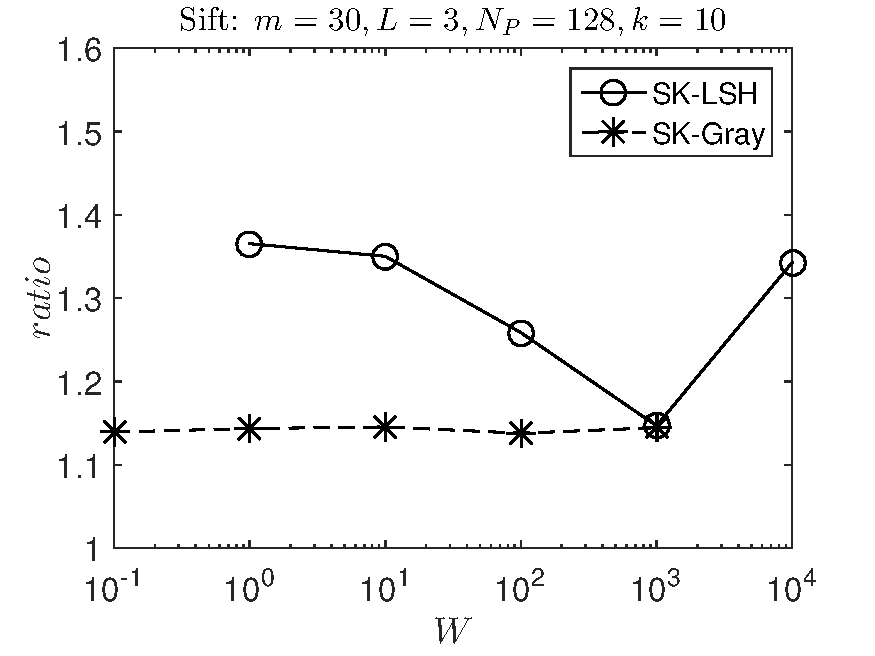
\includegraphics[width=0.45\textwidth]{w_sift.pdf}
			\label{fig:w}
		}
		\subfigure[Comparison of different orders versus $m$]{
			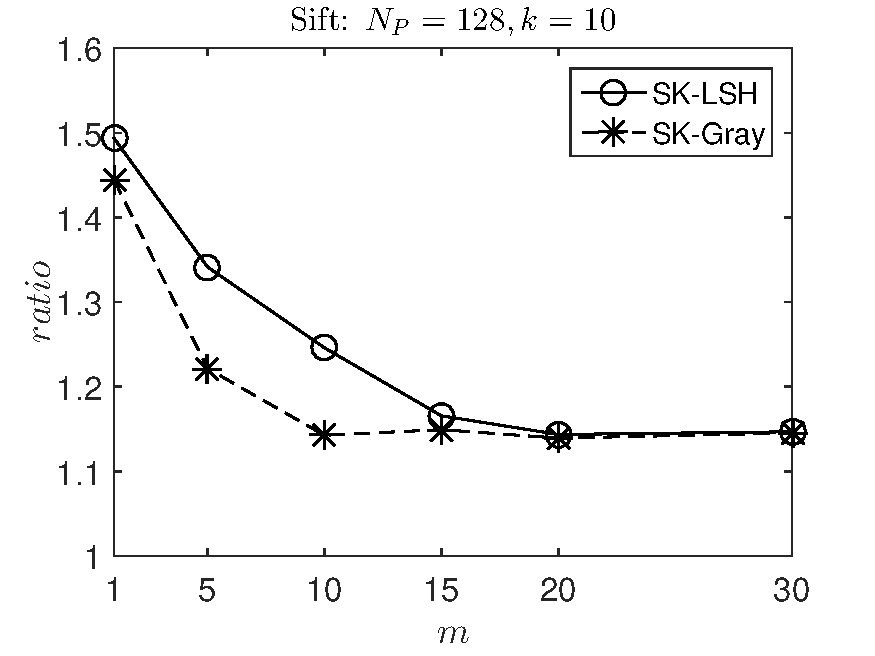
\includegraphics[width=0.45\textwidth]{m_sift.pdf}
			\label{fig:m}
		}		
	\end{center}
	\caption{ANN search comparison on different linear orders}
	\label{fig:ordercomp}
\end{figure*}

% 变化W
Fig. \ref{fig:w} compares the $ratio$ versus different width of LSH functions. Note that we tune $W$ with the ratio of 10 times. It is obviously that SK-LSH is very \emph{sensitive} to $W$. Its accuracy becomes better when the width becomes larger and reaches the optima with a relative large width (in this case, $W$=1000 is the optimal width), after that, it becomes worse again. Relatively, SK-Gray seems not affected by the change of $W$, its accuracy stabilizes at a relatively good level (nearly equal to the optima of SK-LSH). The difference in the sensibility w.r.t $W$ is derived from the different linear orders conducted in these two methods. As analyzed in Section \ref{sssec:anaorder}, the row-wise order is more prone to miss near neighbors during the local traversing due to its dimension-first-traverse property. Enlarging the internal width of LSH functions helps to catch back those missed near neighbors. As for the Gray curve, it will always traverse nearer neighbors first before further areas no matter what the width is, therefore it does need to seek extra help.


% m的变化
A consequence of enlarging $W$ in SK-LSH is that it has to build more LSH functions. Because larger $W$ will enlarge the collision probability of two distant points according to Equation \ref{eq:p(r,w)}, which will bring in more false positives into the candidate set. To protect the accuracy, more LSH functions have to built to adequately filter out these false positives, which finally increases the index and computation overhead. Experiment results in Fig. \ref{fig:m} have corroborated this. As shown, within a certain range, adding LSH functions can help both the methods to improve the ANN search accuracy. The promotion degrades with the growth of $m$ until a certain value after which adding more LSH functions no longer improve the accuracy. That is the optimal $m$ value for each of the method. We see in the figure, SK-LSH has a larger optimal $m$=20 than that of SK-Gray which is 10. 


% inflexion
Note that there is a inflexion in the experiment results in Fig. \ref{fig:w}, when $W$ is larger than 1,000, the $ratio$ of SK-LSH becomes worse again. This is because increasing $W$ will decrease the number of intervals divided along a LSH function. For SK-LSH, $W$ that larger than 1,000 will barely divide no more than 2 intervals which makes all data points mix together according to their compound hash keys.

% conclusion
In conclusion, employing better linear order does help to enhance the local distribution of NN candidates and thus boost the efficiency as well as the algorithm robustness.



\subsection{Performance Comparisons}
In this section, we make thorough comparisons between SC-LSH and four other external methods which are the state-of-the-art LSH-based methods, including C2LSH~\cite{Gan2012C2LSH}, SK-LSH~\cite{Liu2014SKLSH}, SRS~\cite{Sun2014SRS} and QALSH~\cite{Huang2015QALSH}.

\subsubsection{Parameter Settings}\label{sssec:ps}
To make a fair comparison, we set the parameters of each methods to exhibit their best tradeoff on both the accuracy and the I/O efficiency. The detailed parameter settings are listed in Table \ref{tbl:para}.
\begin{table*}[t]
	%\scriptsize
	\centering
	\caption{Parameter settings}\label{tbl:para}
	\begin{tabular}{|c|c|c|c|c|c|}
		\hline
		Datasets & C2LSH & QALSH & SRS & SK-LSH & SC-LSH\\
		\hline
		\textbf{Audio} & $c$=3, $Ct$=1 & $c$=3 & $c$=4 & $m$=10, $W$=3, $\mathcal{L}$=3 & $m$=10, $W$=1, $\mathcal{L}$=3 \\
		\textbf{Sift} & $c$=3, $Ct$=1 & $c$=3 & $c$=4 & $m$=10, $W$=1000, $\mathcal{L}$=3 & $m$=10, $W$=1, $\mathcal{L}$=3 \\
		\textbf{Gist} & $c$=3, $Ct$=1 & $c$=3 & $c$=4 & $m$=10, $W$=2.5, $\mathcal{L}$=3 & $m$=10, $W$=1, $\mathcal{L}$=3\\
		\hline
	\end{tabular}
\end{table*}%
%\normalsize

To some extent, C2LSH and QALSH are similar to each other since they are both based on the dynamic collision counting mechanism. We specify them to achieve different goals. We turn on the early termination condition ($Ct$) in C2LSH to achieve better efficiency, while we let QALSH pursuit better accuracy. As for SRS, we deploy the SRS$-$12 variant and set $c$=4 on all datasets as suggested in~\cite{Sun2014SRS}. For SK-LSH, it needs to tune the parameters to express the best performance, especially the width $W$ of LSH functions. Finally, $W$ are fixed at 3, 1000, 2.5 for Audio, Sift and Gist, respectively. SC-LSH is not sensitive with $W$, in this paper, we fix $W$=1 for all datasets. Actually, in our practical experimental observations, any small value that can divide more than 3$\sim$4 internals along the LSH functions is reasonable for SC-LSH. Besides, we set $m$=10 and $\mathcal{L}$=3 for both SK-LSH and SC-LSH on all the datasets for the sake of fairness.

We vary the number $k$ of the returned nearest neighbor among $\{1,10,20,\ldots,100\}$ to observe the performance trend of all methods for ANN search and list all the experimental results in Fig. \ref{fig:ecomp} and Table \ref{tbl:io} and Table \ref{tbl:spaceconsumption}.

\subsubsection{Accuracy and I/O efficiency}
% ratio的总体排序
\noindent\btitle{Accuracy.} According to Fig. \ref{fig:ratio}, SC-LSH achieves the best accuracy on all datasets, following is QALSH and SK-LSH and then SRS and C2LSH.
% ratio的细节说明
% SC的成功证明了一些观点
The result reflects that the similarity-preserving ability of PQ codes is trustworthy in candidate refining and also demonstrates our opinion that discriminating ability is the key of nearest neighbor discriminating and we are not necessarily relied on the original distance to do candidate refining as discussed in Section \ref{ssec:introPQ}.
% SC精度的一些趋势上的特点
Besides, a characteristic of the ANN search accuracy of SC-LSH is that the accuracy is slightly worse when $k$ is small and becomes better with the growth of $k$. This is caused by the quantization distortion in PQ codes, because nearer neighbors (i.e., when $k$ is small) are more likely to be affected by the quantization distortions compared with further ones.
\begin{figure*}[t]
\begin{center}
\subfigure[Comparison of $ratio$]
{
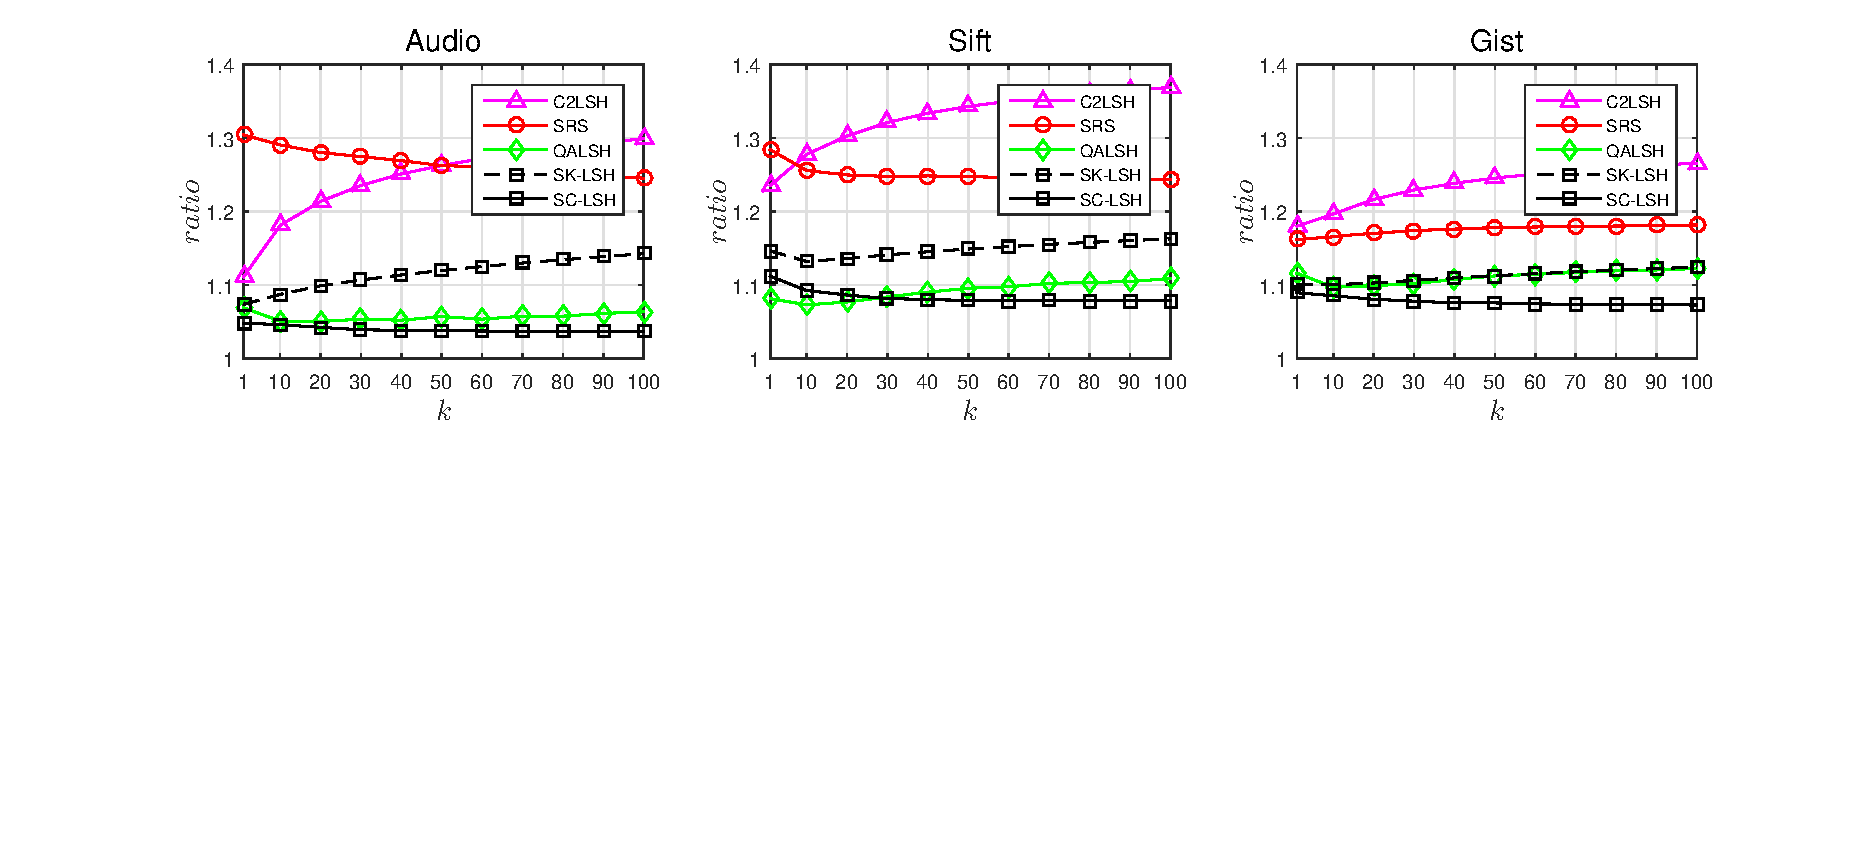
\includegraphics[width=0.98\textwidth]{ratio.pdf}
\label{fig:ratio}
}
\subfigure[Comparison of $I/O$ cost]
{
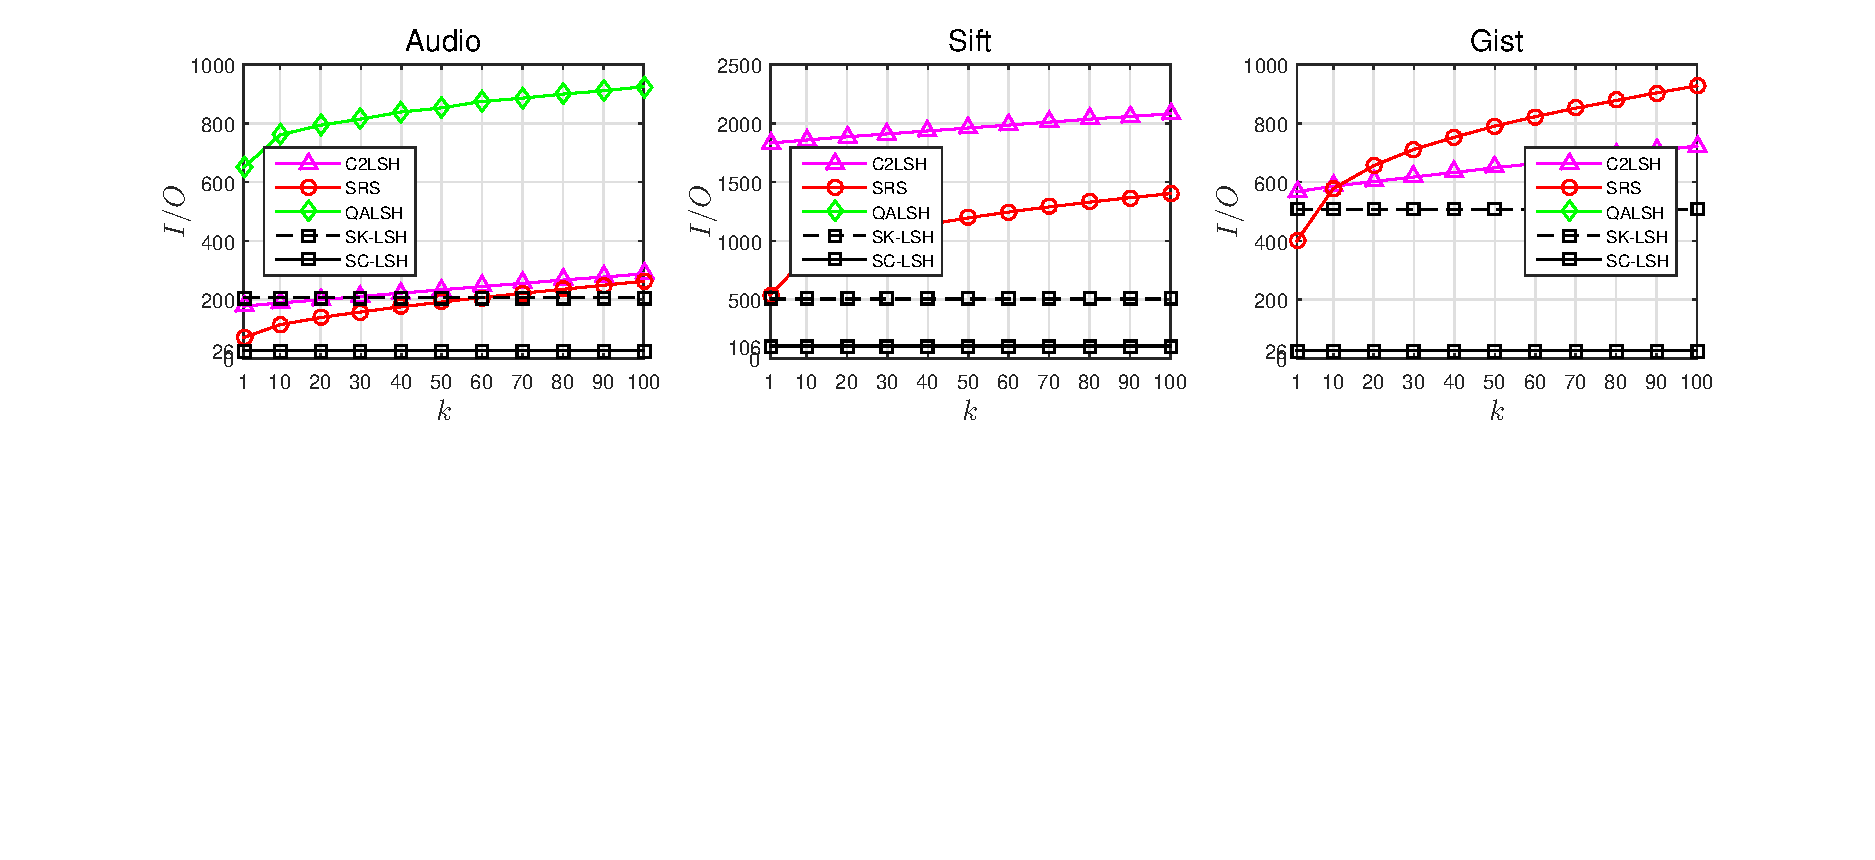
\includegraphics[width=0.98\textwidth]{IO.pdf}
\label{fig:io}
}
\subfigure[Comparison of $ART$]
{
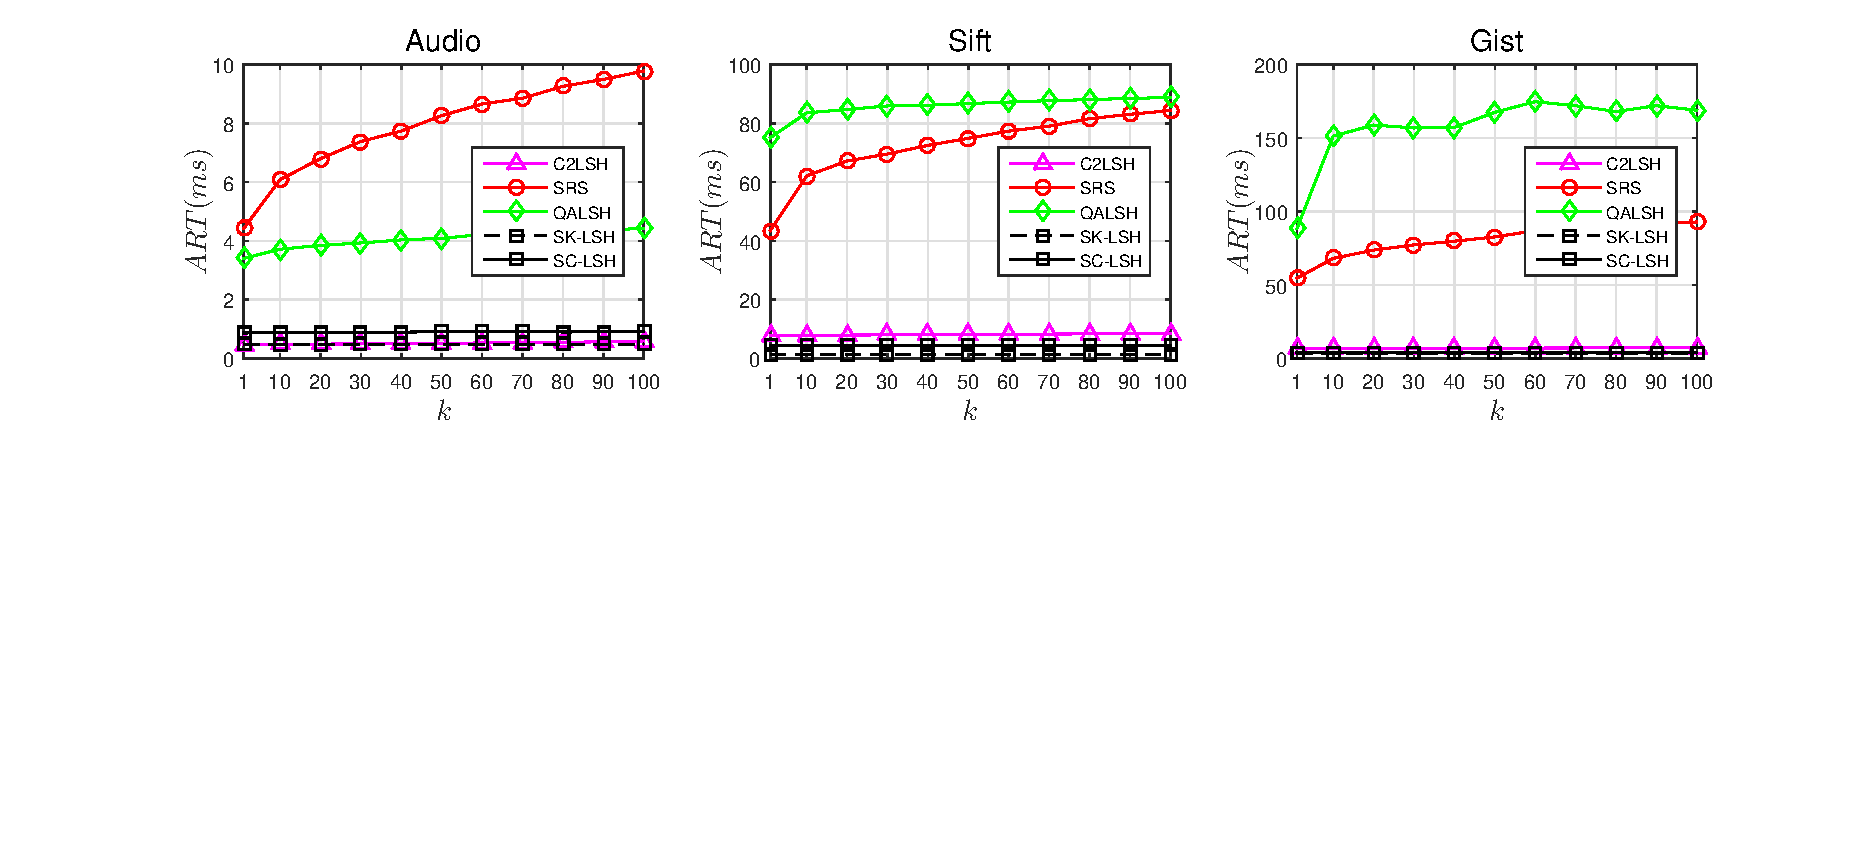
\includegraphics[width=0.98\textwidth]{ART.pdf}
\label{fig:art}
}
\end{center}
\caption{Experimental comparisons}
\label{fig:ecomp}
\end{figure*}

% 总体评价I/O
\noindent\btitle{I/O efficiency.} Considering the I/O cost in Fig. \ref{fig:io}, SC-LSH also achieves the best performance, following is SK-LSH and then SRS and C2LSH. Quantitatively, SC-LSH saves 87\%, 78\% and 95\% I/O operations than SK-LSH respectively on the three datasets. 
% 原因
This is due to the excellent space efficiency of PQ codes, which enables SC-LSH to access sufficiently high quality candidates in much fewer disk page accesses.
% SK-LSH
In contrast, since the candidate capacity of the disk page in SK-LSH is limited by the data dimensionality and usually the disk page size is constant in a certain machine, it has to consume more disk pages in high dimensional datasets. Note that SK-LSH consumes the same amount of I/O operations (i.e., 506) on both Sift and Gist according to Fig. \ref{fig:io}, it seems that SK-LSH is not affected by the data dimensionality. Actually, this is because we set different page size for this two datasets, 4KB for Sift and 16KB for Gist, respectively.
% QA的IO
Besides, we do not draw all the I/O cost of QALSH in Fig. \ref{fig:io}, because it consumes much more I/O operations than the other methods which can be reflected by the results on the Audio dataset in Fig. \ref{fig:io} in a certain extent. Actually, it consumes more I/O operations on other two larger-scaled datasets. We list the numerical results in an extra table (Table \ref{tbl:io}) to better show the difference. As can be seen, on the small-scaled Audio dataset, QALSH consumes 25-35 times more page accesses than SC-LSH. On the two larger datasets, Sift and Gist, the difference grows to 112-133 and 140-166 times, respectively.
\begin{table*}[!htb]
	\centering
	\caption{Comparison of $I/O$ cost between QALSH and SC-LSH}\label{tbl:io}
	\begin{tabular}{|c|c|c|c|c|c|c|c|c|c|}
		\hline
		& \multicolumn{3}{c|}{Audio} & \multicolumn{3}{c|}{Sift} & \multicolumn{3}{c|}{Gist} \\
		\cline{2-10}
		\raisebox{1.2ex}[3pt]{$k$} & QALSH & SC-LSH & Q/S & QALSH & SC-LSH & Q/S & QALSH & SC-LSH & Q/S \\
		\hline
		
		1 & 650 & 26 & 25 & 11901 & 106 & 112 & 3659 & 26 & 140 \\
		10 & 761 & 26 & 29 & 13298 & 106 & 125 & 4052 & 26 & 155 \\
		20 & 794 & 26 & 30 & 13512 & 106 & 127 & 4123 & 26 & 158 \\
		30 & 815 & 26 & 31 & 13646 & 106 & 128 & 4166 & 26 & 160 \\
		40 & 839 & 26 & 32 & 13753 & 106 & 129 & 4192 & 26 & 161 \\
		50 & 853 & 26 & 32 & 13836 & 106 & 130 & 4216 & 26 & 162 \\
		60 & 875 & 26 & 33 & 13926 & 106 & 131 & 4244 & 26 & 163 \\
		70 & 886 & 26 & 34 & 13986 & 106 & 131 & 4268 & 26 & 164 \\
		80 & 900 & 26 & 34 & 14056 & 106 & 132 & 4290 & 26 & 165 \\
		90 & 911 & 26 & 35 & 14128 & 106 & 133 & 4313 & 26 & 165 \\
		100 & 925 & 26 & 35 & 14174 & 106 & 133 & 4332 & 26 & 166 \\
		
		\hline
	\end{tabular}
\end{table*}


% 综合accuracy和IO来看
\noindent\btitle{Accuracy + I/O efficiency.} Considering both the accuracy and I/O efficiency, which are the most two concerned performances in this paper, SC-LSH still performs the best.
% 其他方法:
% QA
QALSH achieves the most proximate accuracy with SC-LSH, sometimes even better (e.g., for some smaller $k$ on Sift), however, it costs the most I/O operations. SK-LSH achieves a relatively good tradeoff between accuracy and I/O efficiency, however, due to the limitation of data dimensionality, it falls back SC-LSH in all these two performances. The SRS method and the early stop version of C2LSH can neither reconcile the contradiction between accuracy and I/O efficiency.


\subsubsection{Time and space consumption}
% 稍微提一下时间开销
As for the $ART$ in Fig. \ref{fig:art}, it shows that SC-LSH is not the fastest, SK-LSH consumes a bit less time than SC-LSH. The reason, we have mentioned in the discussion of the time complexity in Section \ref{ssec:complex}. Although an AQD computation is less expensive than an Euclidean distance computation, SC-LSH takes more verifications under same amount of disk page accesses. For example, on Audio, SK-LSH can get about 1,000 points in 200 pages, while SC-LSH can access nearly 10,000 data codes even in 20 pages.
% QA的IO导致其时间开销是最多的
Besides, the significant I/O consumption leads QALSH to the most ANN search time on Sift and Gist as shown in Fig. \ref{fig:art}.

% space consumption
Table \ref{tbl:spaceconsumption} lists the relative space consumption of all the methods. As can be seen, the maintenance of original datasets has become the dominant storage overhead of the methods. For example, SK-LSH maintains the most copies of original datasets ($\mathcal{L}$=3 in our experiments), as a result, it has the most space consumption among all compared methods. Followed are C2LSH, QALSH and SRS. SRS keeps its leading position in space saving among all the methods maintaining original datasets due to its tiny index structure size. SC-LSH no longer needs original data to do candidate refining, therefore it has the least space consumption. 

\begin{table}[t]
	\centering
	\caption{Comparison of Space Consumption\label{tbl:spaceconsumption}}
	\begin{tabular}{|c|c|c|c|}
		% for Corel dataset
		\hline
		Methods & \textbf{Audio}~(39.3MB) & \textbf{Sift}~(492.01MB) & \textbf{Gist}~(3.58GB) \\
		\hline
		C2LSH & 135MB & 1.43GB & 4.55GB  \\
		\hline
		QALSH & 49MB & 635MB & 3.96GB \\
		\hline
		SRS & 42MB & 537MB & 3.71GB \\
		\hline
		SK-LSH & 121MB & 1.47GB & 10.80GB \\
		\hline
		SC-LSH & 4MB & 103MB & 103MB \\
		\hline
	\end{tabular}
\end{table}%

%{
%\begin{table}[t]
%\centering
%\scriptsize
%\caption{Comparison of Space Consumption\label{tbl:spaceconsumption}}
%\begin{tabular}{|c|c|c|c|c|c|}
%\hline
%Datasets~(size) & C2LSH & QALSH & SRS & SK-LSH & SC-LSH \\
%\hline
%\textbf{Audio}~(39.3MB) & 135MB & 49MB & 42MB & 121MB & 4MB \\
%\hline
%\textbf{Sift}~(492.01MB) & 1.43GB & 635MB & 537MB & 1.47GB & 103MB \\
%\hline
%\textbf{Gist}~(3.58GB) & 4.55GB & 3.96GB & 3.71GB & 10.80GB & 103MB \\
%\hline
%\end{tabular}
%\end{table}
%\normalsize




%======================================================================================================
\section{Related Work}\label{sec:relatedwork}
%======================================================================================================
% NN search的分类
There is a large body of literature on the topic of NN search. Early studies proposed a plenty of work that seek for \emph{exact} nearest neighbors, 
%and lots of tree-based indexings~\cite{Guttman1984,Beckmann1990,White1996,Katayama1997,Berchtold1996,Robinson1981,Bentley1975}
however, all of them suffer from the ``curse of dimensionality"~\cite{Bohm2001,Weber1998}: their running time for NN search degenerate to that of linear scan. Recent developed methods have made some progress in overcoming the dimension curse, such as~\cite{Weber1998,Ferha2000,Jagadish2005iDistance,Ramaswamy2011HB,Feng2017HBPlus,Hwang2012FNN}, etc. However, to guarantee the strict 100\% accuracy, most of them still have to consume large amount of I/O operations and distance computations which makes the efficiency far from satisfactory.

%The most representative approaches in exact NN search include data size reduction such as VA-File~\cite{Weber1998} and its variants IQ-tree~\cite{Berchtold2000}, VA$^{+}$-File~\cite{Ferha2000} and PCVA~\cite{Cui2007}, and one-dimensional transformation such as iDistance~\cite{Jagadish2005} and its improvement~\cite{Shen2005}. Moreover, LDC~\cite{Koudas2004} considers a single-bit representation for each dimension to speed-up the search process. More recently, an idea of reducing both data size and feature dimensionality has also been proposed~\cite{DBLP:conf/sigmod/HuangSLZ11}. In addition, Hyperplane Bounds~\cite{Ramaswamy2011} also reach good enough search performance for correlated high-dimensional datasets, where there exist heavy dependencies across dismension.


% ANN发展概述
Approximate nearest neighbor (ANN) search seeks for high-quality approximate solutions which can fulfill most the query requirements. Without the strict restriction of search accuracy, plenty of effective techniques are developed to promote the search efficiency. Typically, there are three kinds of techniques most developed, which are the hashing techniques, the quantization techniques and the graph based techniques.


\subsection{Hashing techniques}
% hashing based methods
Hashing techniques and in particular locality-sensitive hashing (LSH) have recently gained its popularity in the communities of database and computer vision due to the high efficiency. LSH employs distance-preserving hashing functions to project nearby points into same bucket with high probability which enables fast and accurate irrelevant points filtration with barely no pre-processing. Associated with the construction of compound hash functions and/or multiple hash tables, researchers can effectively reduce the false positives~(FP) and false negatives~(FN).


% basic LSH
The basic LSH methods were first developed in~\cite{Indyk1998LSH,Gionis1999,Datar2004} by Indyk, Gionis and Datar et al. They consume too much space consumption and are only designed for main memory adoption. More works are developed to further boost LSH-based methods.
% 替换 A typical limitation of basic LSH methods is that their indexes require an extremely high amount of space. The original LSH method needs to build hundreds or thousands of hash tables in practice, which is super-linear in the number of data points~\cite{Datar2004}. 
Some of them devote to reduce the space consumption, including Entropy-based LSH~\cite{Panigrahy2006} and Multi-Probe LSH~\cite{Lv2007,Joly2008}. 
% LSB and C2LSH
Tao et al. propose LSB technique~\cite{Tao2009LSB} which is the first LSH method designed for disk-resident data. It generates z-orders with the use of hash keys of compound LSH functions and employs B-trees, called LSB-forest, to manage the index files, which produces a good tradeoff between quality and efficiency. C2LSH~\cite{Gan2012C2LSH} uses \emph{dynamic collision counting} to estimate the actual distances between two points and only a few number of candidates are satisfactory to obtain high-quality results.
% QALSH
Also based on the dynamic collision counting mechanism, QALSH introduces a concept of \emph{query-aware} bucket partition which uses the query as the ``anchor" for bucket partition after the query arrives so that to remove the random shift in the traditional \emph{query-oblivious} projection.
% SRS
SRS aimes at reducing the index size, it uses only 6 random projections to convert high-dimensional data into low dimensions so that they can be indexed by a single tiny index.
% SK-LSH
Most the above methods unavoidably need to consume large number of random I/Os for candidates collecting, SK-LSH proposes a sorting-keys strategy to address this. It introduces space linear order into compound hash keys to enhance the local distribution of candidates which improves the disk access manner as well as loading more high-quality candidates during a single page access. However, this measure unfortunately endures poor scalability with high dimensions. Since the page size $B$ is usually constant, as the dimensionality grows, less candidates can be held in a single disk page, which obliges it ultimately resort for more disk page access to guarantee the search accuracy.

% LSB 与 SK-LSH对我们方法的启发
In fact, the LSB technique is the first one who exploits linear order to estimate the similarity between data points. But it mainly emphasizes on how to boost the ANN accuracy and does not provide further measurements on how to optimize I/O operations as what SK-LSH does. Nevertheless, thanks to their instructive work. It is during the exploring of the difference between row-wise curve and z-ordering where we come to realize the difference effects on the local arrangement of candidates between DFT orders and NFT ones.

% LSH方法精简描述 The basic LSH method was first proposed by M. Datar~\cite{Datar2004}. But it consumes too much space consumption. Several methods were proposed to reduce the space consumption, including Entropy-based LSH~\cite{Panigrahy2006} and Multi-Probe LSH~\cite{Lv2007,Joly2008}. LSB~\cite{Tao2009} generates z-orders with the use of hash keys of compound LSH functions and employs B-trees, called LSB-forest, to manage the index files, which produces a good tradeoff between quality and efficiency. C2LSH~\cite{Gan2012} uses \emph{dynamic collision counting} to estimate the actual distances between two points and only a few number of candidates are satisfactory to obtain high-quality results. Note that there also exist many machine learning based hashing methods~\cite{DBLP:conf/cvpr/HeoLHCY12,DBLP:conf/sigmod/Song13}. However, they usually require an expensive learning process to learn hash functions which could be highly data-dependent.


% SK-LSH的线序与LSB的线序
% Some others attempt to improve the I/O efficiency by  as well as elevating the candidate hit rate of a single page access in order to reduce the total I/O operations.
% SK-LSH第一个这么做,线序组织、提取代表键值,定义键值距离,限制I/O 次数等一系列措施。SK-LSH (short for SortingKeys-LSH) is the first LSH-based method that specifically devote to optimize the I/O efficiency. It introduces a linear order to rearrange the data points so that candidates can be stored locally and thus be loaded continuously within less page access. During the ANN search, it strictly limits the number of disk page permitted to access, and also defines several distance measurements between the query data and disk pages to better guide the ANN search. However, it encounters several drawbacks


% learn-based LSH
% Note that there also exist many machine learning based hashing methods~ \cite{DBLP:conf/cvpr/HeoLHCY12,DBLP:conf/sigmod/Song13}. However, they usually require an expensive learning process to learn hash functions which could be highly data-dependent.


\subsection{Quantization techniques}
% PQ 通过压缩空间占用,加入内存,提升效率。但是搜索方式有些粗糙。
Quantization techniques, especially product quantization~\cite{Jegou2011PQ,Norouzi2013} are increasingly popular in the community of computer vision. They encode all points with a product quantizer and compute \emph{asymmetric quantizer distances (AQD)} between codes of query and data points during the search process. Finally, the data point with the smallest AQD value is returned as the ANN of the query. The basic PQ method was proposed by H. Jegou et al.~\cite{Jegou2011PQ} and has been improved by several works~\cite{Babenko2012Inverted,Norouzi2013,WangWSXSL15,Yannis2014LOPQ} since then. In particular, M. Norouzi et al.~\cite{Norouzi2013} proposed CK-Means, which improves the accuracy of returned results by optimally rotating the original space and re-ordering the dimensions.

% PQ系列方法在内存,我们探讨外存中PQ码的应用
Although PQ codes are initially designed for internal memory, we explore its potential in external memory in this paper to sharpen our index for ANN search. Thanks to PQ-based technique, SC-LSH is now insensitive to the dimensionality of dataset. It can verify much more candidate points than~\cite{Liu2014SKLSH} within the same or even less number of I/O accesses. As a result, SC-LSH can preserve similar, or even dramatically higher, accuracy under fewer I/O operations. We hope that our exploration can provide valuable references for future research.

\subsection{Graph based techniques}
% graph based methods
% 基本原理,基本问题
There is another series of work based on neighborhood graph. Neighborhood graph (or nearest neighbor graph, NNG) is a directed graph that connects each data point to its nearest neighbors. Searching in a neighborhood graph is often proceeded by a local neighborhood graph search procedure that incorporates various heuristic rules such as best-first strategy or priority queue. A fundamental limitation of the local search is that the search process may enter into local optima. 
% 办法的研究分两种
Mainly two kinds of efforts are devoted to alleviate this problem. The first one focuses on optimizing the search strategy, including improving the initial candidate neighbors~\cite{Hajebi2009AkNNG,Jin2014NNE} or better guiding the iterated neighborhood graph expansion~\cite{Wang2012Query,WangJD2013NNGPQ,Malkov2016HNSW,Fu2016EFANNA}. Another efforts reside in sharpening the neighborhood graph construction. Building a k-nearest neighbor graph (k-NNG) is the most direct way to approximate the Delaunay graph which can maintain efficient exploration costs by limiting the degree of each vertex in the graph~\cite{Dong2011kNNG,Paredes2006kNNG}. Approximate k-nearest neighbor graph~\cite{Hajebi2009AkNNG,Ponomarenko2011,Gan2012ScalablekNNG,Zhang2013FastkNNG} provides an alternative approach to approximate the k-NNG which can offer a significant speed-up for the offline graph building. Besides, there are some other methods seek for adaptively neighbor connecting method in order to exploit some of the intrinsic structure of the dataset~\cite{Malkov2014SmallWorld,HarwoodD2016FANNG}. 
  
% 总体评价
Overall, graph-based techniques have made significant progress in boosting the ANN search accuracy but have also left over two main issues. Firstly, computational cost of constructing neighborhood graph is usually very large which should be treated cautiously. Besides, routing on the neighborhood graph relied on original distances, the access of data points are all consumed in random I/Os.

% 一个特别提出的工作
Some of the latest work also concern about the I/O performance boosting of external ANN search methods. A representative one is made by Tang et al. who manage to reduce the candidate refining time as well as the I/O cost by exploiting caching techniques of compact approximate representations of data points in main memory, which is orthogonal to our work~\cite{Tang2016Exploit}.



%======================================================================================================
%\vspace{-3ex}
\section{Conclusion}\label{sec:conclusion}
%======================================================================================================
In this paper, we propose a novel LSH index structure, SC-LSH, to further boost the ANN search accuracy together with the I/O efficiency. We exploit the Gray curve with neighbor-first-traverse property as the order of compound hash keys sorting to enhance the local distribution of NN candidates and thus boost the ANN search efficiency as well as the algorithm robustness. Storing compact binary codes (specifically PQ codes) instead of original data points to do candidate refining can significantly reduce the I/O cost, and extensive experiments conducted on real-life datasets demonstrate the ability of PQ codes for NN discriminating and also the superiority of SC-LSH over the other compared LSH approaches.


\begin{acknowledgements}
This work is supported by National Natural Science Foundation of China (Nos. 61472298, 61672408, 61702403, U1135002), National High Technology Research and Development Program (863 Program, No.2015AA016007), China 111 Project (No. B16037), Natural Science Basic Research Plan in Shaanxi Province of China (Program No. 2015JQ6227), SRF for ROCS, SEM and the Fundamental Research Funds for the Central Universities (JB170308).
\end{acknowledgements}

\begin{acknowledgements}
	This work is supported by National Natural Science Foundation of China (Nos. 61472298, 61672408, 61702403, U1135002), National High Technology Research and Development Program (863 Program, No.2015AA016007), China 111 Project (No. B16037), Natural Science Basic Research Plan in Shaanxi Province of China (Program No. 2015JQ6227), SRF for ROCS, SEM and the Fundamental Research Funds for the Central Universities (JB170308).
\end{acknowledgements}

% BibTeX users please use one of
%\bibliographystyle{spbasic}      % basic style, author-year citations
\bibliographystyle{spmpsci}      % mathematics and physical sciences
%\bibliographystyle{spphys}       % APS-like style for physics
\bibliography{cuiref}   % name your BibTeX data base
 

\end{document}
% end of file template.tex

